\documentclass[12pt, dvipdfmx]{beamer}

\renewcommand{\kanjifamilydefault}{\gtdefault}
%%%%%%%%%%%  package  %%%%%%%%%%%
\usepackage{bxdpx-beamer}% dvipdfmxなので必要
\usepackage{pxjahyper}% 日本語で'しおり'したい

\usepackage{amssymb,amsmath,ascmac}

% \usepackage{multirow}
\usepackage{bm}

\graphicspath{{../../../figures/}}

\usepackage{tikz}
\usepackage{xparse}

\usepackage{multimedia}

\usetikzlibrary{shapes,arrows}
%% define fancy arrow. \tikzfancyarrow[<option>]{<text>}. ex: \tikzfancyarrow[fill=red!5]{hoge}
\tikzset{arrowstyle/.style n args={2}{inner ysep=0.1ex, inner xsep=0.5em, minimum height=2em, draw=#2, fill=black!20, font=\sffamily\bfseries, single arrow, single arrow head extend=0.4em, #1,}}
\NewDocumentCommand{\tikzfancyarrow}{O{fill=black!20} O{none}  m}{
\tikz[baseline=-0.5ex]\node [arrowstyle={#1}{#2}] {#3 \mathstrut};}

%微分関連のマクロ
%
\newcommand{\diff}{\mathrm d}
\newcommand{\difd}[2]{\dfrac{\diff #1}{\diff #2}}
\newcommand{\difp}[2]{\dfrac{\partial #1}{\partial #2}}
\newcommand{\difdd}[2]{\dfrac{\diff^2 #1}{\diff #2^2}}
\newcommand{\difpp}[2]{\dfrac{\partial^2 #1}{\partial #2^2}}
\newcommand{\rmd}{\mathrm{d}}
\newcommand{\dd}[1]{\dfrac{\mathrm{d} #1}{\mathrm{d} x}}

%目次スライド
\AtBeginSection[noframenumbering]{
  \frame{\tableofcontents[currentsection]}
}

%アペンディックスのページ番号除去
\newcommand{\backupbegin}{
   \newcounter{framenumberappendix}
   \setcounter{framenumberappendix}{\value{framenumber}}
}
\newcommand{\backupend}{
   \addtocounter{framenumberappendix}{-\value{framenumber}}
   \addtocounter{framenumber}{\value{framenumberappendix}} 
}



%%%%%%%%%%%  theme  %%%%%%%%%%%
\usetheme{Copenhagen}
% \usetheme{Metropolis}
% \usetheme{CambridgeUS}
% \usetheme{Berlin}

%%%%%%%%%%%  inner theme  %%%%%%%%%%%
% \useinnertheme{default}

% %%%%%%%%%%%  outer theme  %%%%%%%%%%%
\useoutertheme{default}
% \useoutertheme{infolines}

%%%%%%%%%%%  color theme  %%%%%%%%%%%
%\usecolortheme{structure}

%%%%%%%%%%%  font theme  %%%%%%%%%%%
\usefonttheme{professionalfonts}
%\usefonttheme{default}

%%%%%%%%%%%  degree of transparency  %%%%%%%%%%%
%\setbeamercovered{transparent=30}

% \setbeamertemplate{items}[default]

%%%%%%%%%%%  numbering  %%%%%%%%%%%
% \setbeamertemplate{numbered}
\setbeamertemplate{navigation symbols}{}
\setbeamertemplate{footline}[frame number]

%%%%%%%%%%%%%%%%%%%%%%%%%%%%%%%%%%%
\title
[ランダムな接続性を有するネットワークポリマーの緩和挙動]
{ランダムな接続性を有する\\ネットワークポリマーの緩和挙動}
\author[東亞合成 佐々木]{佐々木裕}
\institute[東亞合成]{東亞合成}
\date{Desember 16, 2022}
%%%%%%%%%%%%%%%%%%%%%%%%%%%%%%%%%%
\begin{document}

\setlength{\abovedisplayskip}{2pt} % 上部のマージン
\setlength{\belowdisplayskip}{2pt} % 下部のマージン

%%%%%%%%%%%%%%%%%%%%%%%%%%%%%%%%%%
\begin{frame}[noframenumbering]\frametitle{}
	\titlepage
\end{frame}
% %%%%%%%%%%%%%%%%%%%%%
% \section*{}
% %
% \begin{frame}
% %[allowframebreaks]
% {Outline}
% 	\tableofcontents
% \end{frame}

%%%%%%%%%%%%%%%%%%%%%
\section{はじめに}

\subsection{本研究の目標とアプローチ}
\begin{frame}
    \frametitle{本研究の目標とアプローチ}
        \begin{block}{目標}
                \begin{itemize}
                    \item 高分子材料の破壊耐性向上の設計指針を得たい。
                    \item 耐久性、可逆性に優れた材料として、\\
					\alert{ゴム材料(柔らかいネットワーク)}をターゲット
                \end{itemize}
        \end{block}
		\begin{exampleblock}{アプローチ}
            \begin{itemize}
                \item 実験的アプローチ
                \begin{itemize}
                    \item 超分子前駆体から構造明確な\alert{三分岐}ネットワーク
                    \item フィラー無添加での\alert{高い破断伸びと強度}
                    \item 既知のモデルとの多数の整合点と、\alert{よくわからない点}。
                \end{itemize}
                \item シミュレーションでモデルを構築
                \begin{itemize}
                    \item 単純化したモデルで小さなスケールから始めたい。
                    \item \alert{長さの揃ったストランドで MD シミュレーション}
                    % \item 最終的に、亀裂先端の挙動を FEM シミュレーション
                \end{itemize}
            \end{itemize}
		\end{exampleblock}
\end{frame}

\subsection{ゴムの強靭性}
\begin{frame}
	\frametitle{ゴム系材料の破壊とヒステリシスロス}
	\vspace{-1mm}
		% \begin{block}{}
			\begin{columns}[T, onlytextwidth]
				\column{.63\linewidth}
					\begin{itemize}
						\item ヒステリシスロス
							\begin{itemize}
								\item 変形履歴による力学応答変化
								\item サイクル変形でエネルギー散逸
							\end{itemize}
						\item 破壊エネルギーと\alert{正の相関}\footnote{
								\scriptsize{K.A.Grosch, J.A.C.Harwood, A.R.Payne, \\Rub. Chem. Tech., 41, 1157(1968)}
							}
							\begin{itemize}
								\item \alert{変形温度}にも強く依存
								\item ガラス転移温度との距離?
							\end{itemize}
						\item ヒステリシスロス発生の起源\footnote{
							\scriptsize{A.R.Payne, J.Poly.Sci.:Sympo., 48, 169(1974)}
						}
						\begin{itemize}
							\item \alert{粘弾性に基づくもの}
							\item 結晶化に由来するもの
							\item 添加したフィラーに起因
						\end{itemize}
					\end{itemize}
				\column{.35\linewidth}
				\begin{center}
					\vspace{-2mm}
					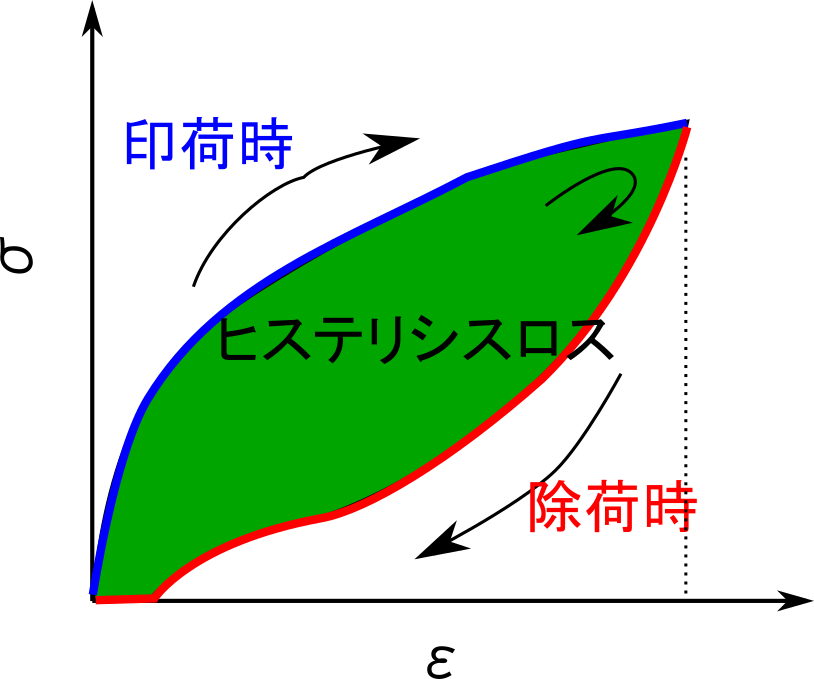
\includegraphics[width=\textwidth]{hysteresis_curve.png}

					\vspace{5mm}
					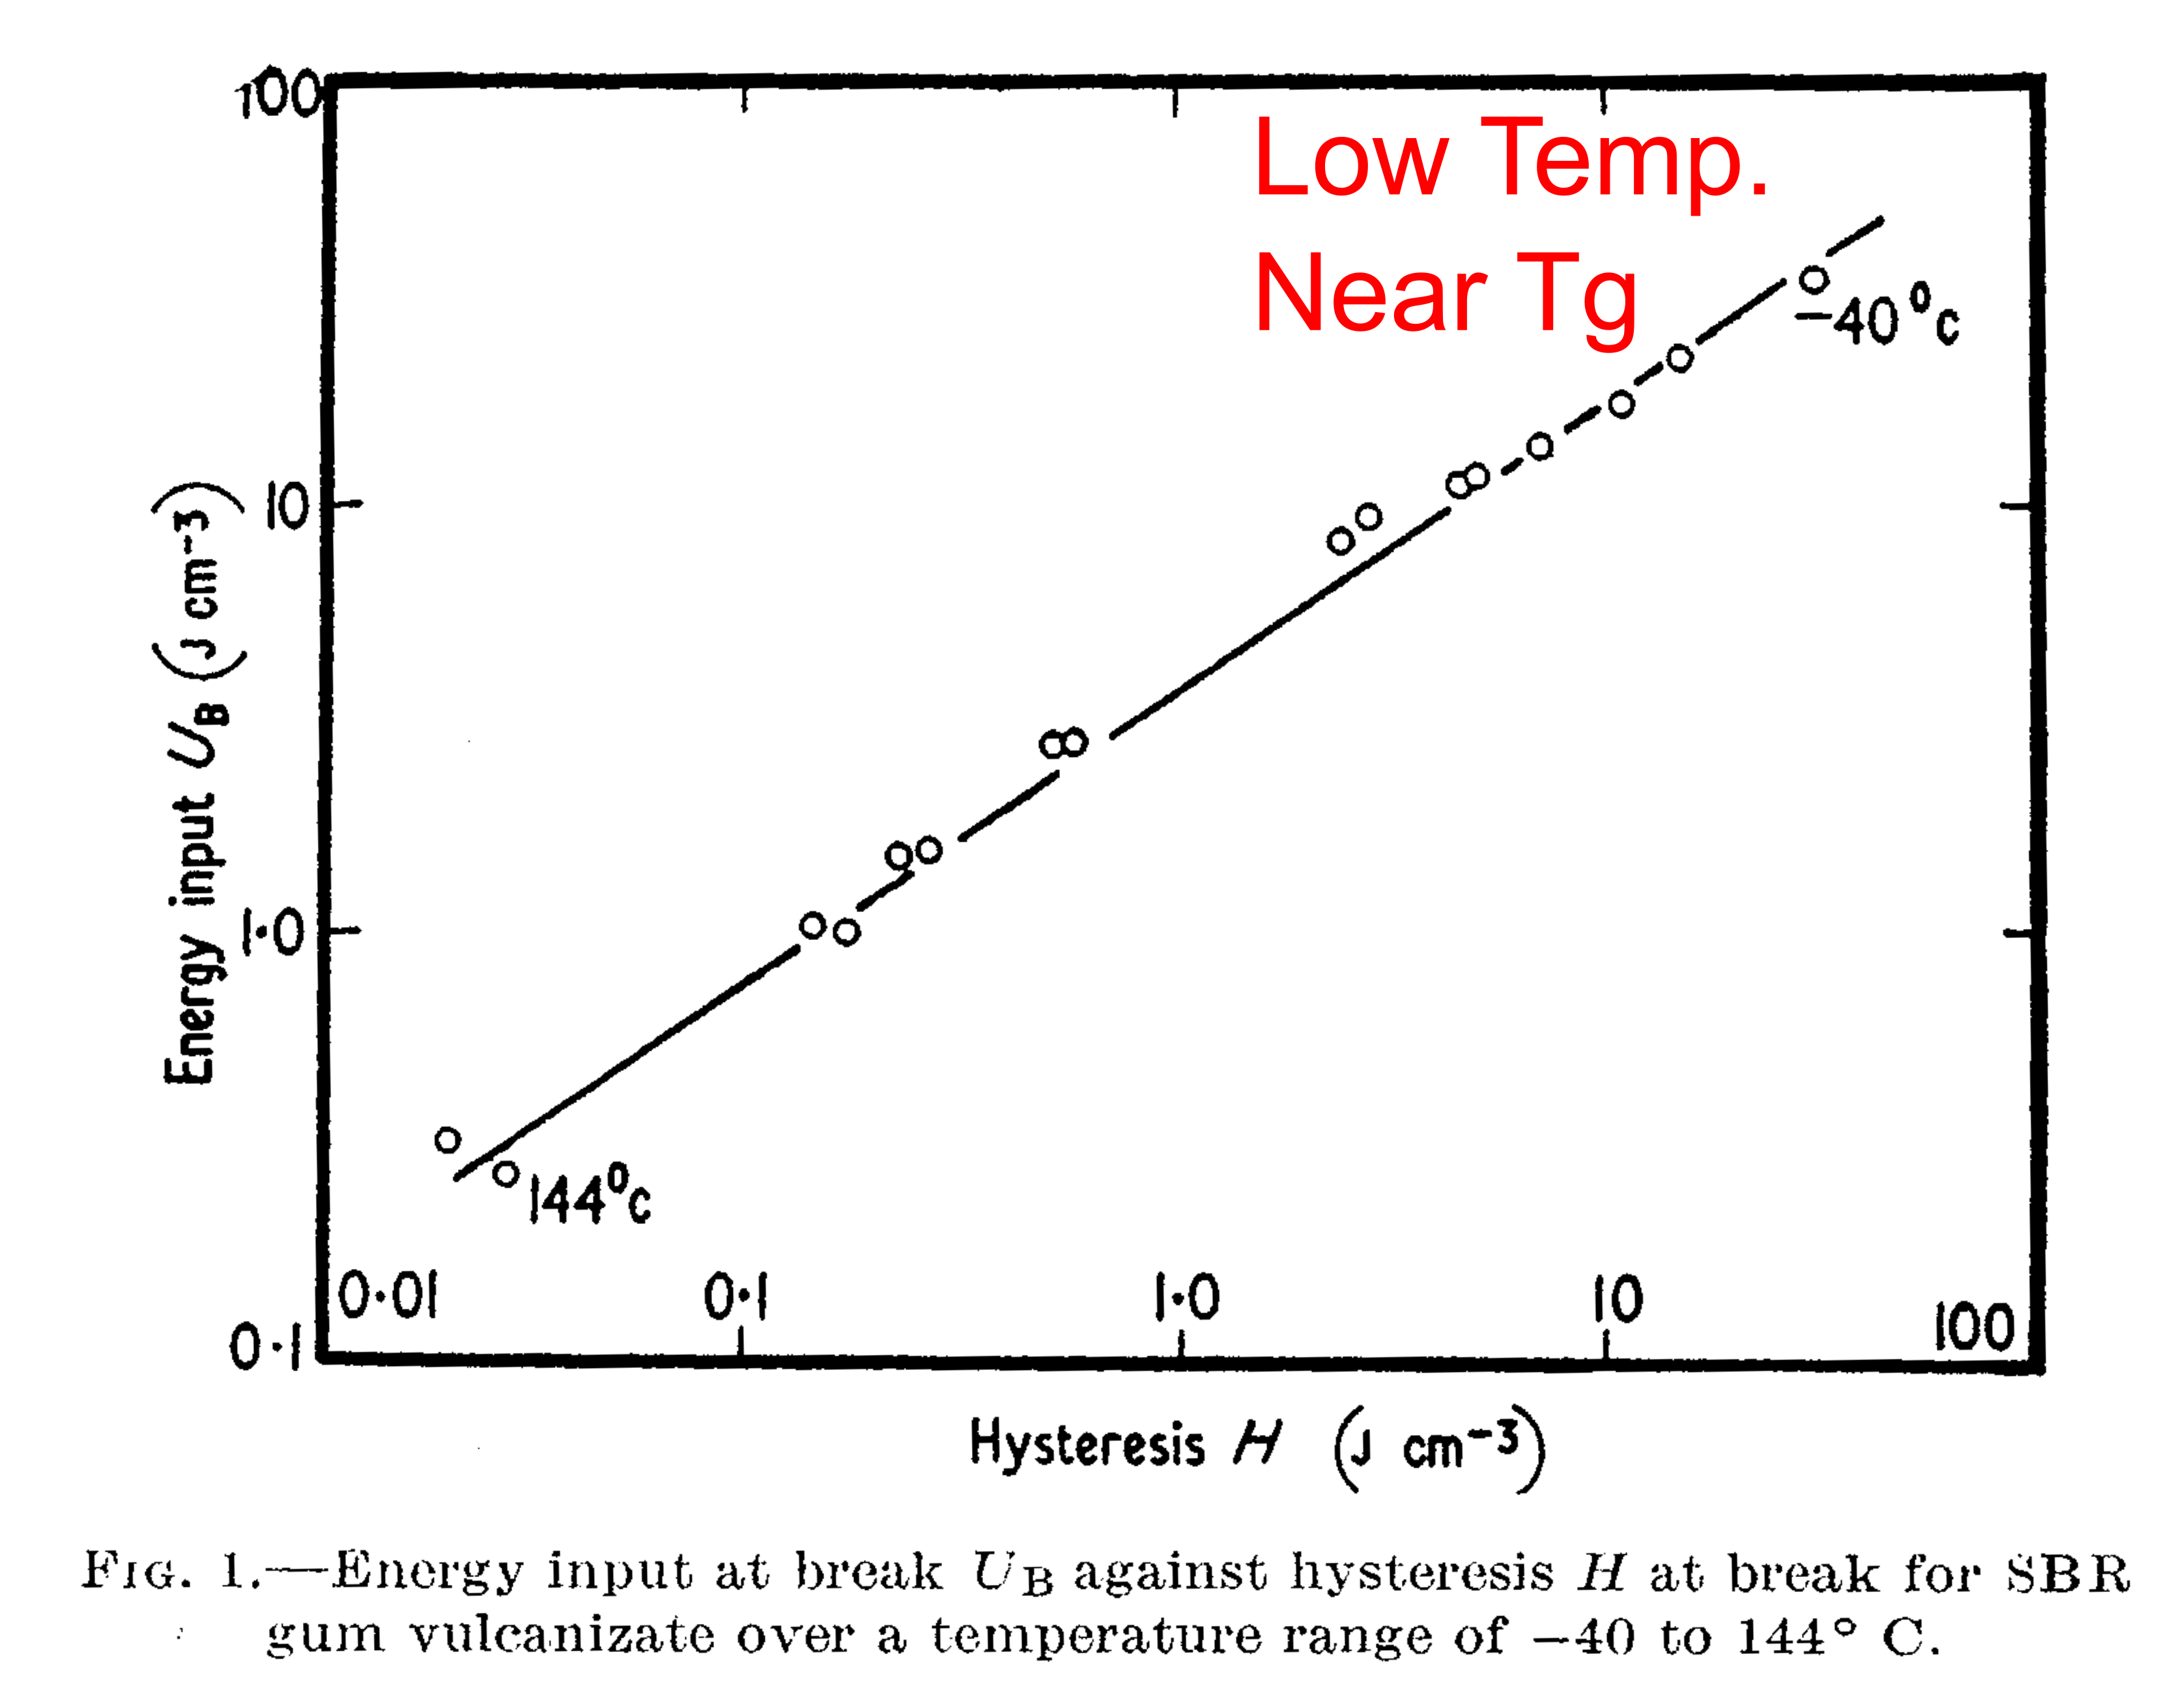
\includegraphics[width=\textwidth]{hyst_break2.png}
				\end{center}
			\end{columns}
		% \end{block}
\end{frame}

\begin{frame}
	\frametitle{ゴムの破壊と時間温度換算則}
		\begin{alertblock}{ゴムの破壊について}
			クラック先端での大変形を伴う非線形現象だが、\\時間温度換算則の成立が多数報告\footnote{
				Smith T., Stedry P., J. Appl. Phys., 31 1892 (1960)
			}
		\end{alertblock}
		\vspace{-2mm}
		\begin{columns}[T, totalwidth=\textwidth]
			\column{.48\textwidth}
				亀裂先端近傍での大変形
				\vspace{-3mm}
				\begin{center}
					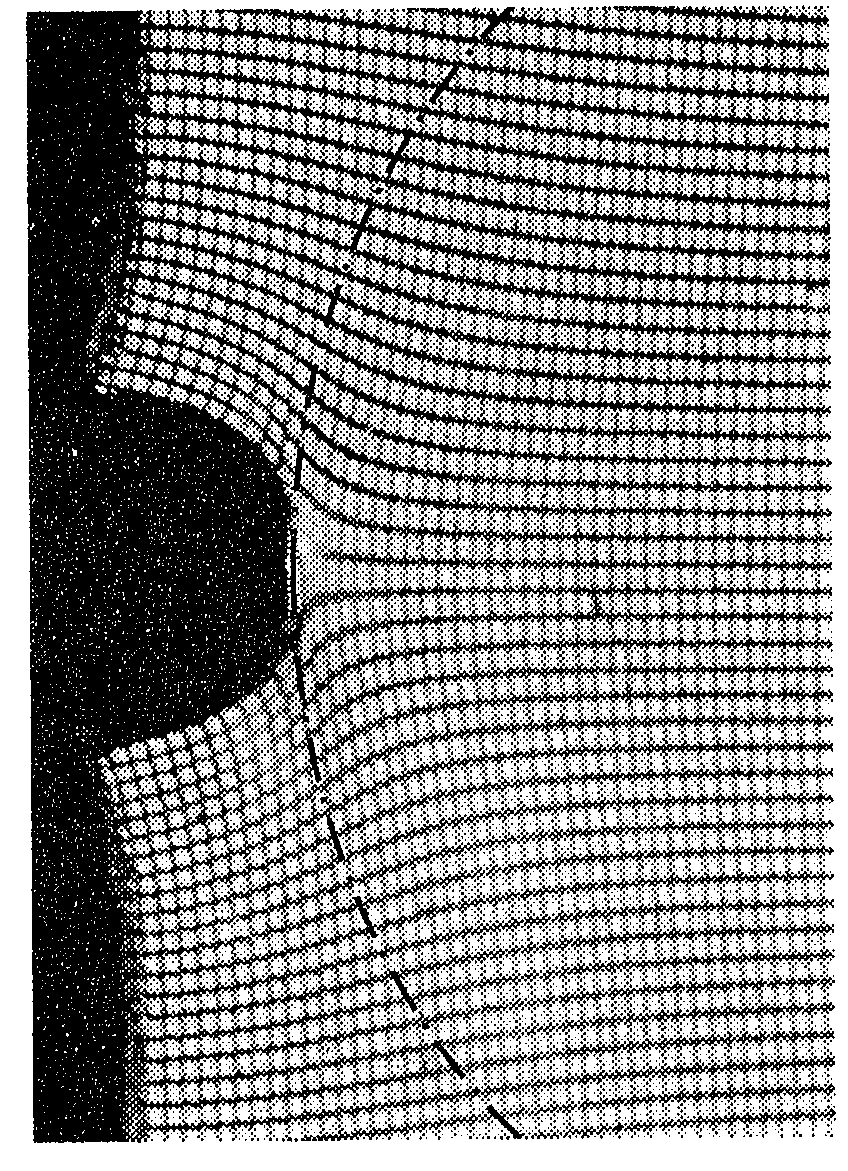
\includegraphics[width=.55\textwidth]{rubber_crack.png}
				\end{center}
			\column{.48\textwidth}
				時間温度換算則の成立
				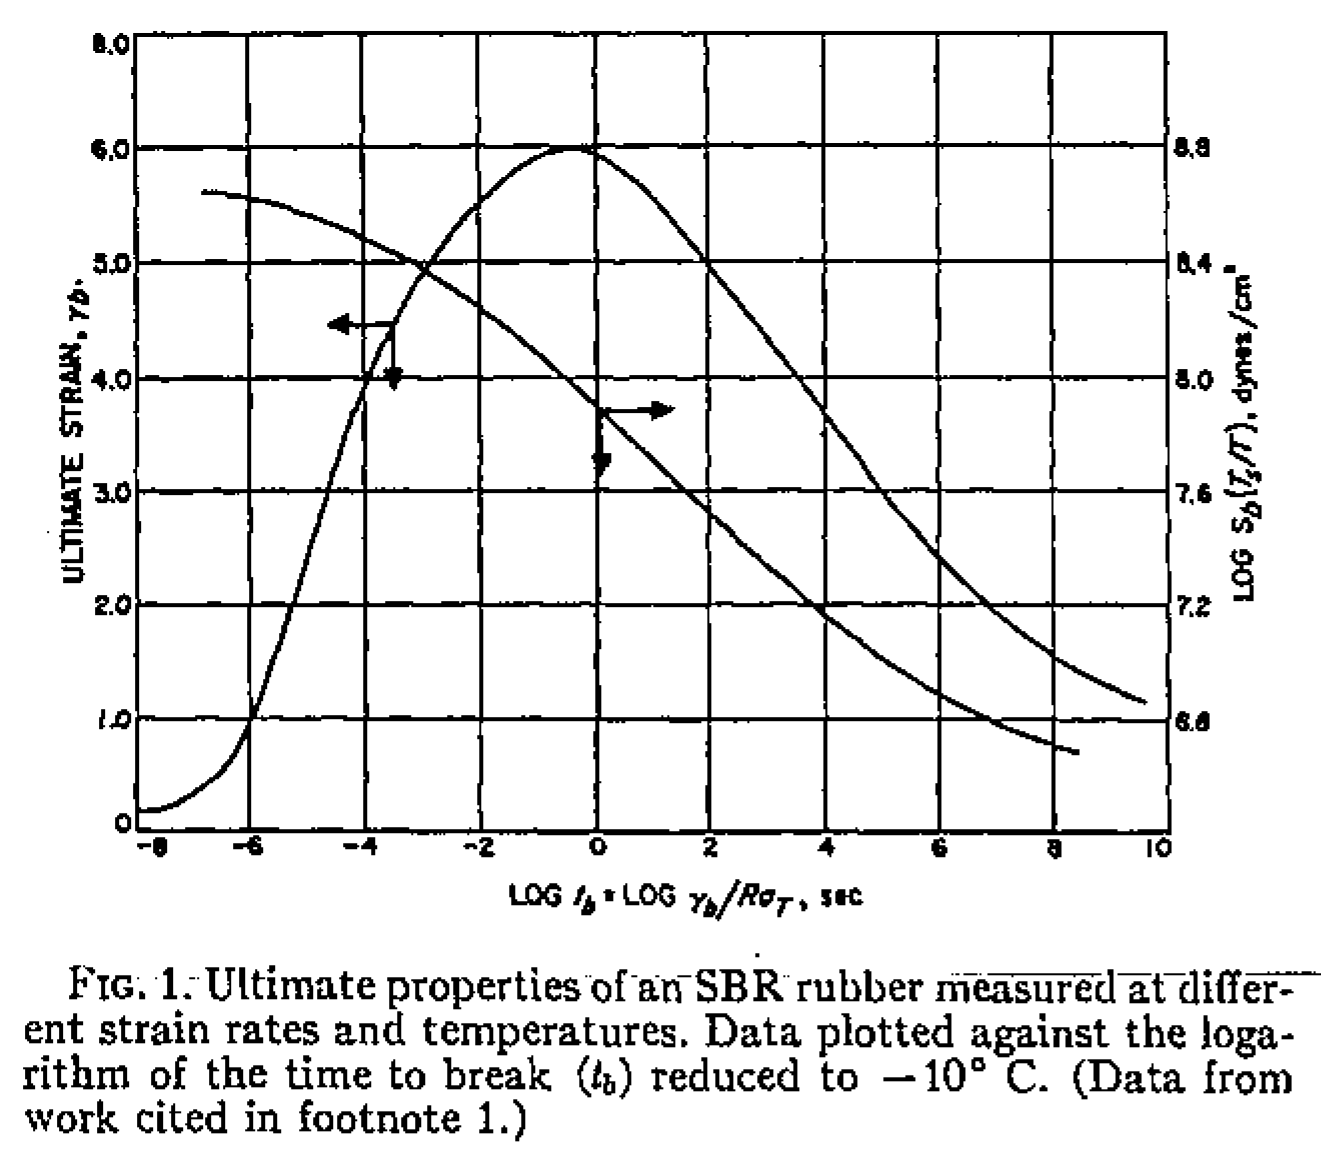
\includegraphics[width=.8\textwidth]{Time_Temp_2.png}
		\end{columns}
\end{frame}

\begin{frame}
	\frametitle{SBRでの伸びきり効果}
		\begin{alertblock}{室温で伸び切りが出ないはずのSBR}
			\begin{itemize}
				\item \alert{低温、高速変形}でSBRでも伸びきり効果が発現\footnote{
					{\footnotesize Smith TL., Dickie RA., J. Pol. Sci. part A-2 (1969) 7 635}
				}
				\item 時間温度換算則で考えてみれば?
			\end{itemize}

			\centering
			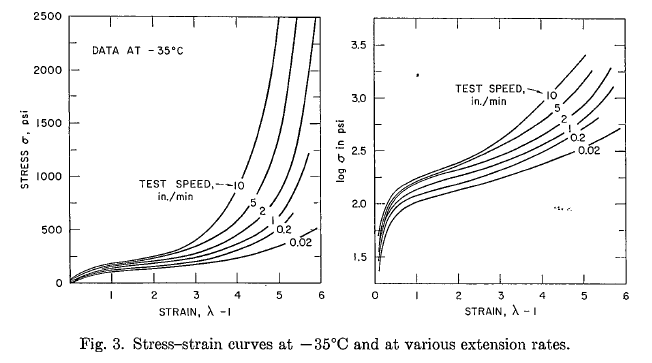
\includegraphics[width=.6\textwidth]{SBR_lowTemp_2.png}
		\end{alertblock}
\end{frame}

\begin{frame}
	\frametitle{ゴムの強靭性}
	% \vspace{-2mm}
		\begin{exampleblock}{Andrews 理論}
			\begin{columns}[T, onlytextwidth]
				\column{.75\linewidth}
				\begin{itemize}
					\item クラック近傍の応力場に注目\footnote{
						\scriptsize
			{E.H.Andrews, Y.Fukahori, J. of Mat. Sci. 12, 1307 (1977)}
					}
						\begin{itemize}
							\item \color{blue}{Loading 場}と \color{red}{Unloading 場}
						\end{itemize}
					\item クラック進展時に\color{green}{応力場が遷移}
						\begin{itemize}
							\item ヒステリシスロス$\Rightarrow${エネルギー散逸}
							\item クラックの進展を\alert{抑制}
						\end{itemize}
				\end{itemize}
				\column{.25\linewidth}
					\begin{center}
						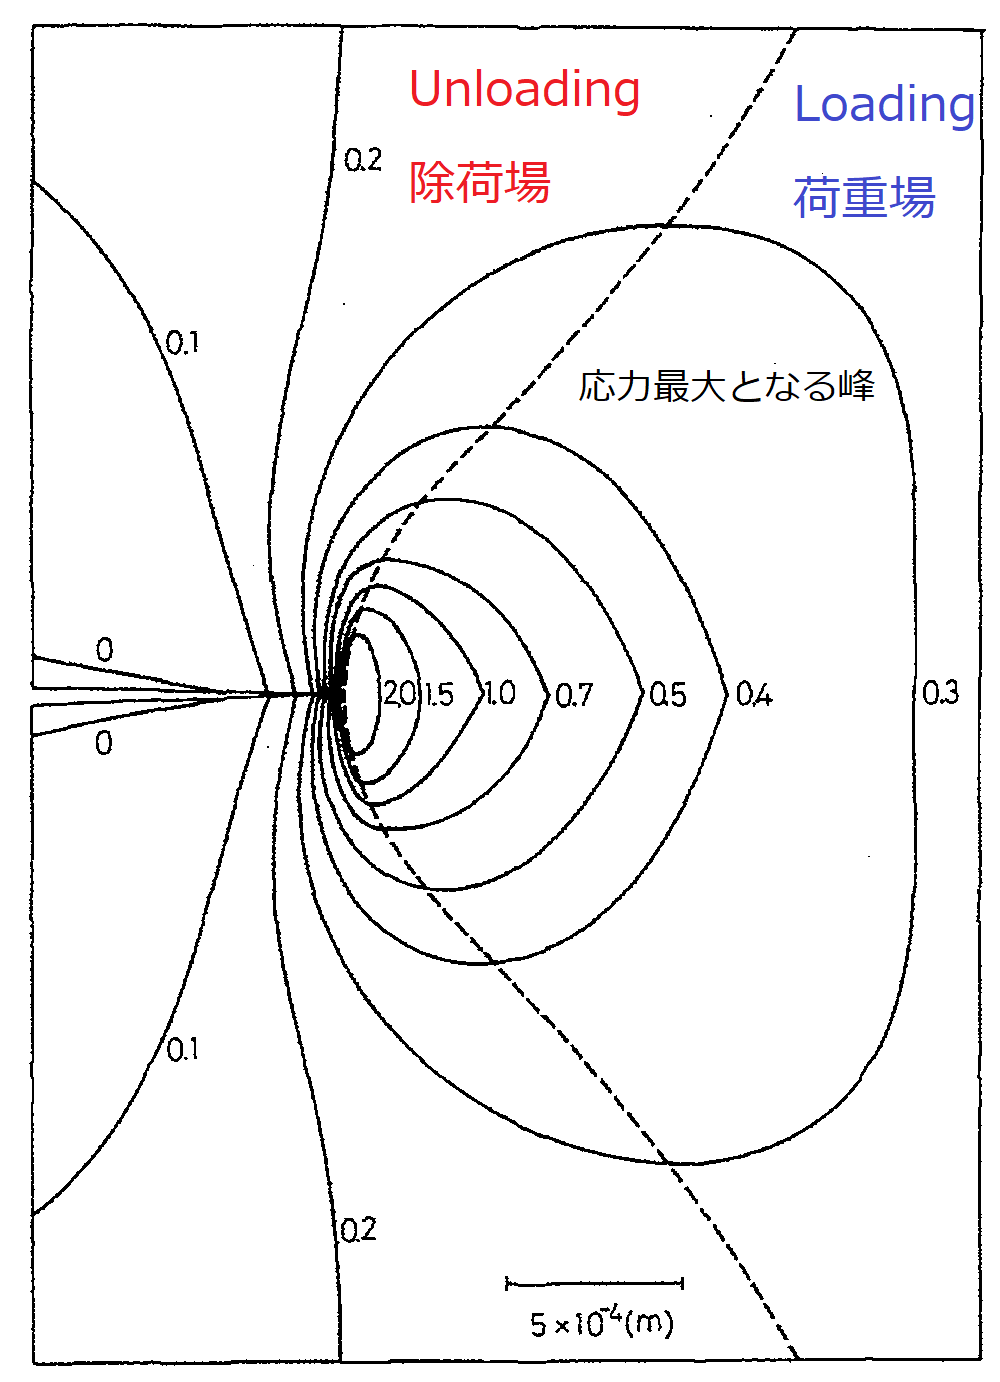
\includegraphics[width=.85\textwidth]{crack.png}
					\end{center}
			\end{columns}
		\end{exampleblock}
		\vspace{-2mm}
		\begin{alertblock}{疲労破壊も考慮すると}
			\begin{itemize}
				\item \alert{可逆的}であることが望ましい。\textcolor{blue}{$\neq$ 犠牲結合}
				\item 変形の周期に対応できるように、\alert{回復速度}も重要。
				\item 粘弾性挙動としてのヒステリシスロス$\Leftrightarrow$緩和挙動
			\end{itemize}
		\end{alertblock}
\end{frame}

\subsection{ゴムのモデル化}
\begin{frame}
    \frametitle{Classical Theory of Rubber Elasticity}
        \vspace{-2mm}
		\begin{block}{Free Energy Density of Rubbers against Strain invariant}
			\vspace{-2mm}
			% 非圧縮性条件から第3不変量がおちて、
			\scriptsize
			\begin{align*}
				\dfrac{F}{V} = W 
				% &= \sum_{i,j = 0}^{\infty} C_{ij}(I_1-3)^i(I_2-3)^j \\[-2mm]
				&= C_0 + {\color{green}C_1(I_1-3)} + C_2(I_2-3) + {\color{red}\sum_{i,j = 1}^{\infty} C_{ij}(I_1-3)^i(I_2-3)^j}
			\end{align*}  
		\end{block}
		\vspace{-5mm}
		\begin{columns}[T, onlytextwidth]
			\column{.48\linewidth}
				\begin{exampleblock}{Neo-Hookean Model}
					\vspace{-2mm}
					% 第1不変量のみを対象
						\scriptsize
						\begin{align*}
							&W = C_1 (I_1-3) \\
							&\text{against Uniaxial elongation} \\
							&\sigma_{nom} = 2 C_1\left(\lambda - \dfrac{1}{\lambda^2}\right) = G \left(\lambda - \dfrac{1}{\lambda^2}\right)
						\end{align*}
				\end{exampleblock}
			\column{.48\linewidth}
				\begin{alertblock}{Mooney-Rivlin Model}
					\vspace{-2mm}
					% 高次の項をおとす
					\scriptsize
					\begin{align*}
						&W = C_1 (I_1-3) + C_2(I_2-3) \\
						&\text{against Uniaxial elongation} \\
						&\sigma_{nom} = 2 \left(C_1 + C_2\dfrac{1}{\lambda} \right) \left(\lambda - \dfrac{1}{\lambda^2}\right)
					\end{align*}
				\end{alertblock}
		\end{columns}
		\vspace{-1mm}
		\begin{block}{With or without Junction Poinits fluctuation}
			\vspace{1mm}
			\begin{columns}[T, onlytextwidth]
				\column{.48\linewidth}
				\small
				\color{blue}{Affine Network Model
				\footnote{
					\tiny{P.J. Flory, Principles of Polymer Chemistry, (1953)}
				}
				}
				\vspace{-2mm}
				\scriptsize
				\begin{align*}
					% &\text{Affine Network Model}\\
					&G_{affine} = \nu k_B T  \\
					&\text{$\nu$: Number density of strands in the system}
				\end{align*}
				\column{.48\linewidth}
				\small
				\color{magenta}{Phantom Network Model
				\footnote{
					\tiny{H.M. James, E.J. Guth, Chem. Phys., 21, 6, 1039 (1953)}
				}
				}
				\vspace{-2mm}
				\scriptsize
				\begin{align*}
					% &\text{Phantom Network Model}\\
					&G_{phantom} = \nu k_B T \left(1 - \dfrac{2}{f}\right) \\
					&\text{$f$: Functionality of Junction Points}
				\end{align*}
				\normalsize
			\end{columns}
		\end{block}
\end{frame}

\begin{frame}
	\frametitle{Constraint Factors for Junction Points and Strands}
		\vspace{-2mm}
		\begin{alertblock}{Vicinity of Junction Point}
			\begin{columns}[totalwidth=1\textwidth]
				\column{.72\textwidth}
				\vspace{-3mm}
				\begin{itemize}
					\item Junction points are \alert{surrounded by many of adjacent strands(x in fig.).}
					\item Because of surrounding strands, \alert{fluctuation of junctions are suppressed}. 
				\end{itemize}
				\column{.25\textwidth}
				\centering
				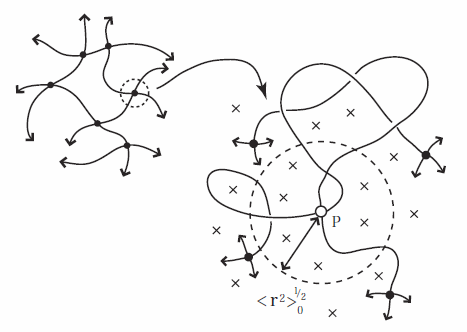
\includegraphics[width=\textwidth]{JP_vicinity.png}
			\end{columns}
		\end{alertblock}
		\vspace{-2mm}
		% \begin{block}{Constraind Junction Model}
		% 	\vspace{-2mm}
			\begin{columns}[totalwidth=1\textwidth]
				\column{.65\textwidth}
				\begin{itemize}
					\item Constraind Junction Model
					\begin{itemize}
						\item With increased strain, constraints are reduced and act as PNM.\footnote{\tiny{P.J.Flory, J.Chem.Phys., 66, 12, 5720 (1977)}}
					\end{itemize}
					\item Topological relationships
					\begin{itemize}
						\item Contribution of entanglement.\footnote{\tiny{D.S.Pearson and W.Graessley, Macromol., 11, 3, 528 (1978)}}
						\vspace{-2mm}
						\begin{align*}
							G_e = T_e G_N^0
						\end{align*}
					\end{itemize}
				\end{itemize}
				\column{.32\textwidth}
				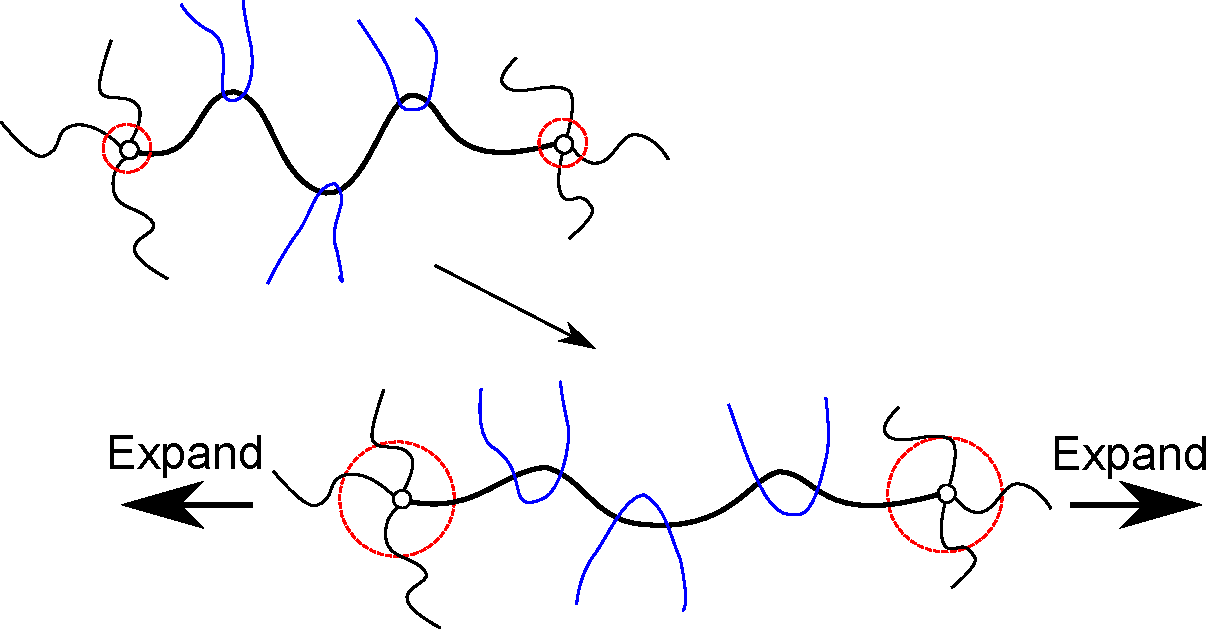
\includegraphics[width=\textwidth]{Constrained_Juntion.pdf}

				\vspace{5mm}
				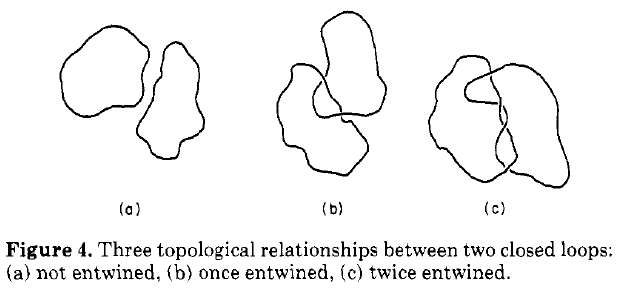
\includegraphics[width=\textwidth]{topological_effect_ring.png}
			\end{columns}
		% \end{block}
\end{frame}

% \begin{frame}
% 	\frametitle{Resent approach for Constraints(Entanglements)}
% 		\vspace{-2mm}
% 		\begin{alertblock}{Slip-tube Model}
% 			\begin{columns}[totalwidth=1\textwidth]
% 				\column{.7\textwidth}
% 				\small
% 				\begin{itemize}
% 					\item Diffused-Constraint Model
% 					\small
% 					\begin{itemize}
% 						\item Confining potential affect all points along the chain.\footnote{\tiny{A. Kloczkowski, J.E. Mark, B. Erman, Macromol., 28, 5089 (1995)}}
% 					\end{itemize}
% 					\item Nonaffine Tube Model
% 					\small
% 					\begin{itemize}
% 						\item Improved model of "Edwards’ Tube Model".\footnote{\tiny{M. Rubinstein, S. Panyukov, Macromol., 30, 25, 8036 (1997)}}
% 					\end{itemize}
% 					\item Slip-tube Model
% 					\small
% 					\begin{itemize}
% 						\item Like slip-link models, a pairwise interaction of chains.\footnote{\tiny{M. Rubinstein, S. Panyukov, Macromol., 35, 6670 (2002)}}
% 					\end{itemize}
% 				\end{itemize}
% 				\scriptsize
% 				\begin{align*}
% 					&f^*(\lambda^{-1}) = G_c + \dfrac{G_e}{0.74 \lambda + 0.61 \lambda^{-1/2} - 0.35} \\
% 					&G_c = \nu k_B T \left(1-\dfrac{2}{\phi} \right), \quad G_e = \dfrac{4}{7} \nu k_B T L
% 					% &\text{where $\nu$ is the number density of network chains,} \\
% 					% & \text{and L is the number of slip-links per network chain}
% 				\end{align*}
% 				\column{.25\textwidth}
% 				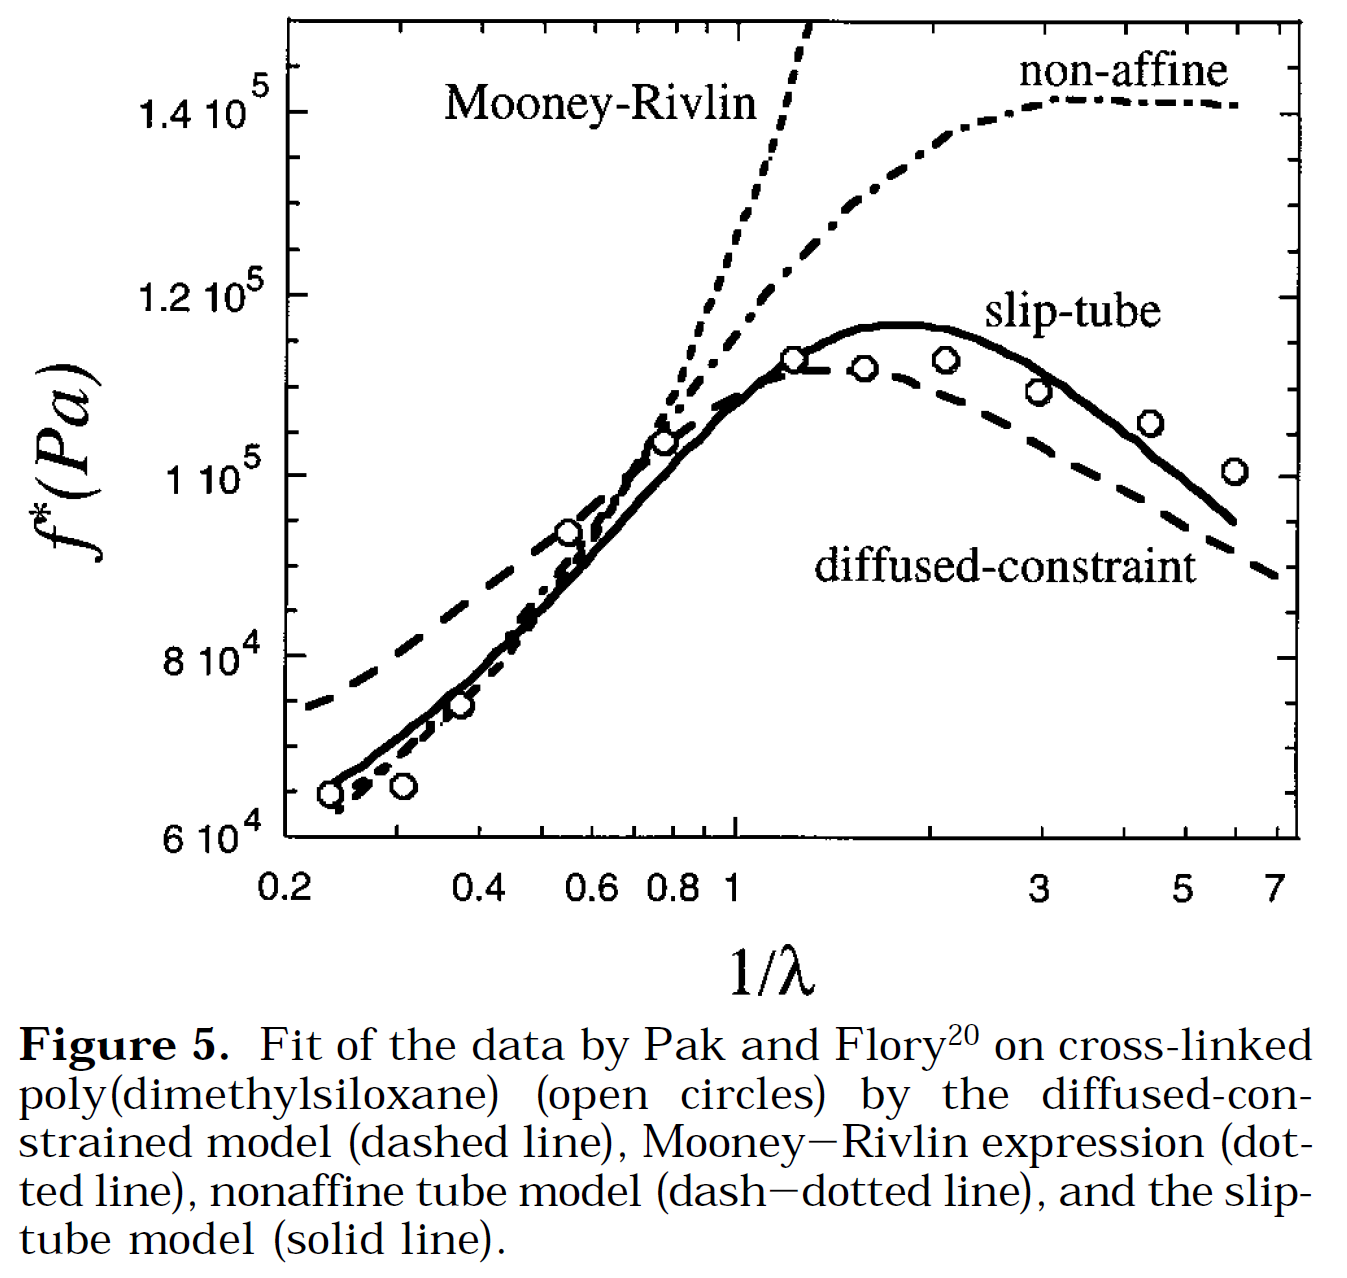
\includegraphics[width=\textwidth]{NW_model_rubinstein.png}
% 			\end{columns}
% 		\end{alertblock}
% \end{frame}


\begin{frame}
	\frametitle{Resent approach for Constraints(Entanglements)}
	
		\begin{itemize}
			\item Diffused-Constraint Model
			\begin{itemize}
				\item Confining potential affect all points along the chain.\footnote{\tiny{A. Kloczkowski, J.E. Mark, B. Erman, Macromol., 28, 5089 (1995)}}
			\end{itemize}
			\item Nonaffine Tube Model
			\begin{itemize}
				\item Improved model of "Edwards' Tube Model".\footnote{\tiny{M. Rubinstein, S. Panyukov, Macromol., 30, 25, 8036 (1997)}}
			\end{itemize}
			\item Slip-tube Model
			\begin{itemize}
				\item A pairwise interaction of chains is introduced.\footnote{\tiny{M. Rubinstein, S. Panyukov, Macromol., 35, 6670 (2002)}}
			\end{itemize}
		\end{itemize}

		\begin{alertblock}{Slip-tube Model(Simple analytical appoximation)}
			\begin{columns}[totalwidth=1\textwidth]
				\column{.7\textwidth}
				\scriptsize
				\begin{align*}
					&f^*(\lambda^{-1}) = G_c + \dfrac{G_e}{0.74 \lambda + 0.61 \lambda^{-1/2} - 0.35} \\
					&G_c = \nu k_B T \left(1-\dfrac{2}{\phi} \right), \quad G_e = \dfrac{4}{7} \nu k_B T L \\
					% &\text{where $\nu$ is the number density of network chains,} \\
					& \text{L is the number of slip-links per network chain}
				\end{align*}
				\column{.25\textwidth}
				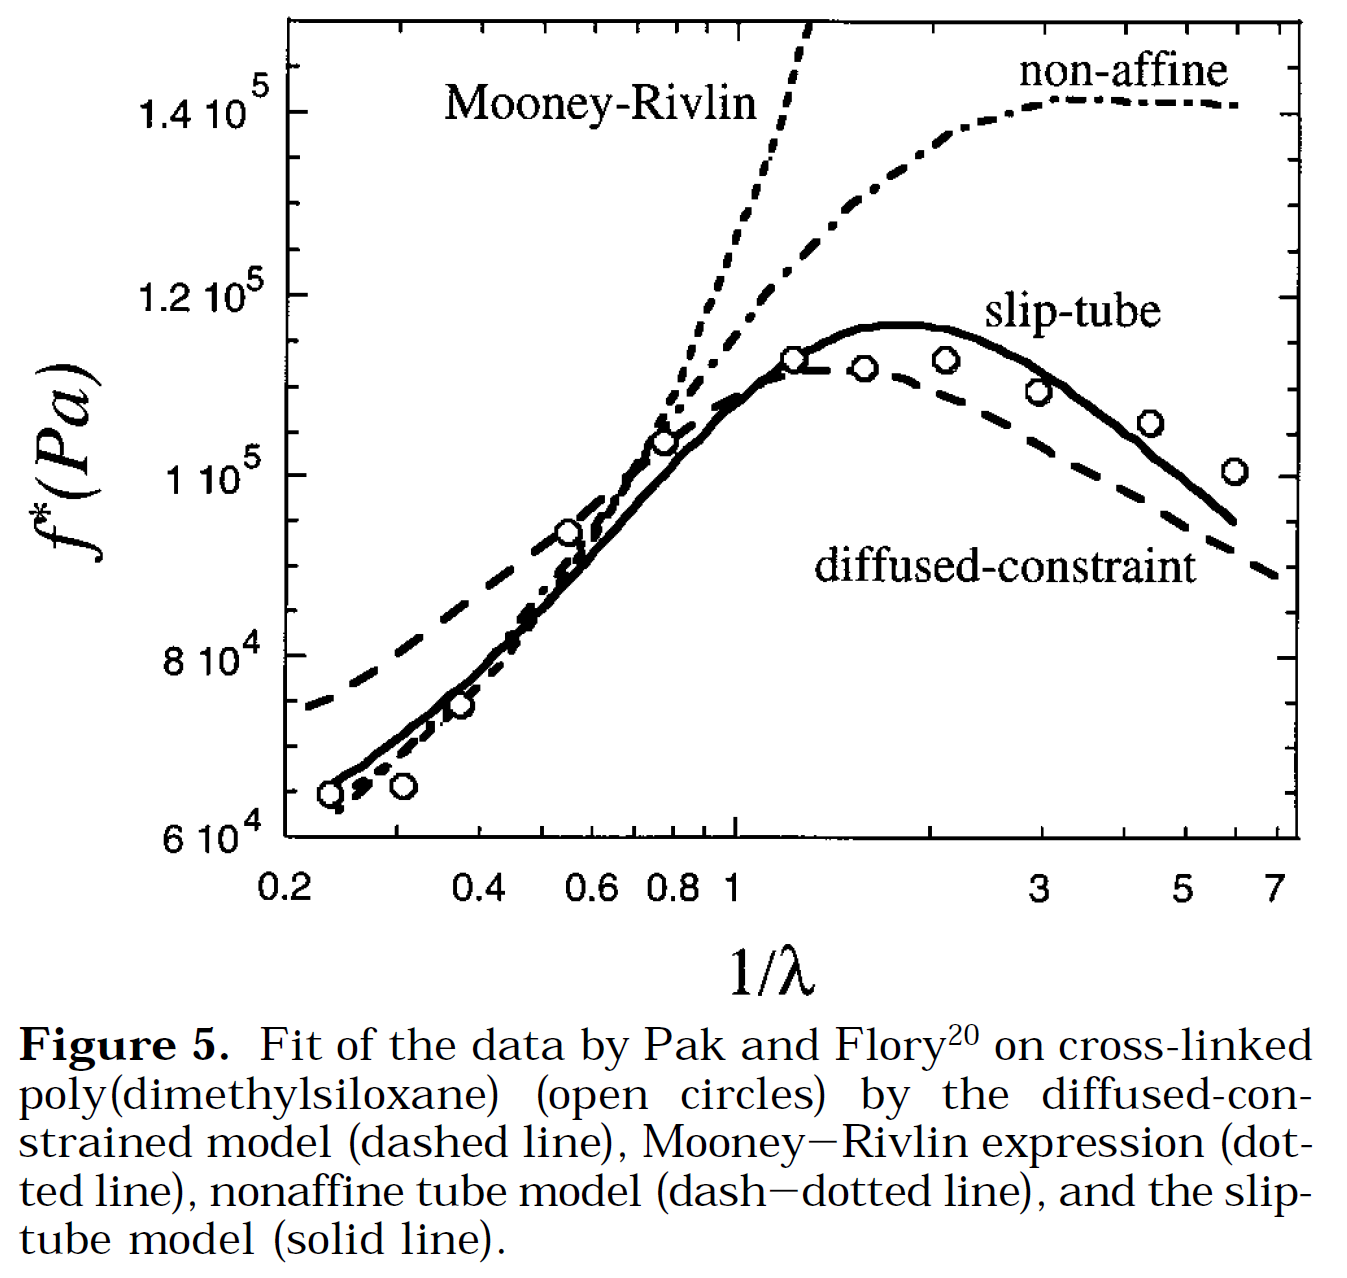
\includegraphics[width=.9\textwidth]{NW_model_rubinstein.png}
			\end{columns}
		\end{alertblock}	
\end{frame}

% \begin{frame}
% 	\frametitle{Resent approach for Constraints(Entanglements)}
	
		

% 		\begin{alertblock}{Slip-tube Model}
% 			\begin{itemize}
% 				\item Diffused-Constraint Model
% 				\begin{itemize}
% 					\item Confining potential affect all points along the chain.\footnote{\tiny{A. Kloczkowski, J.E. Mark, B. Erman, Macromol., 28, 5089 (1995)}}
% 				\end{itemize}
% 				\item Nonaffine Tube Model
% 				\begin{itemize}
% 					\item Improved model of "Edwards' Tube Model".\footnote{\tiny{M. Rubinstein, S. Panyukov, Macromol., 30, 25, 8036 (1997)}}
% 				\end{itemize}
% 				\item Slip-tube Model
% 				\begin{itemize}
% 					\item A pairwise interaction of chains is introduced.\footnote{\tiny{M. Rubinstein, S. Panyukov, Macromol., 35, 6670 (2002)}}
% 				\end{itemize}
% 			\end{itemize}
% 		\end{alertblock}	
% 		\begin{columns}[T, onlytextwidth]
% 			\column{.7\textwidth}
% 			\scriptsize
% 			\begin{align*}
% 				&f^*(\lambda^{-1}) = G_c + \dfrac{G_e}{0.74 \lambda + 0.61 \lambda^{-1/2} - 0.35} \\
% 				&G_c = \nu k_B T \left(1-\dfrac{2}{\phi} \right), \quad G_e = \dfrac{4}{7} \nu k_B T L\\
% 				% &\text{where $\nu$ is the number density of network chains,} \\
% 				% & \text{L is the number of slip-links per network chain}
% 			\end{align*}
% 			\column{.25\textwidth}
% 			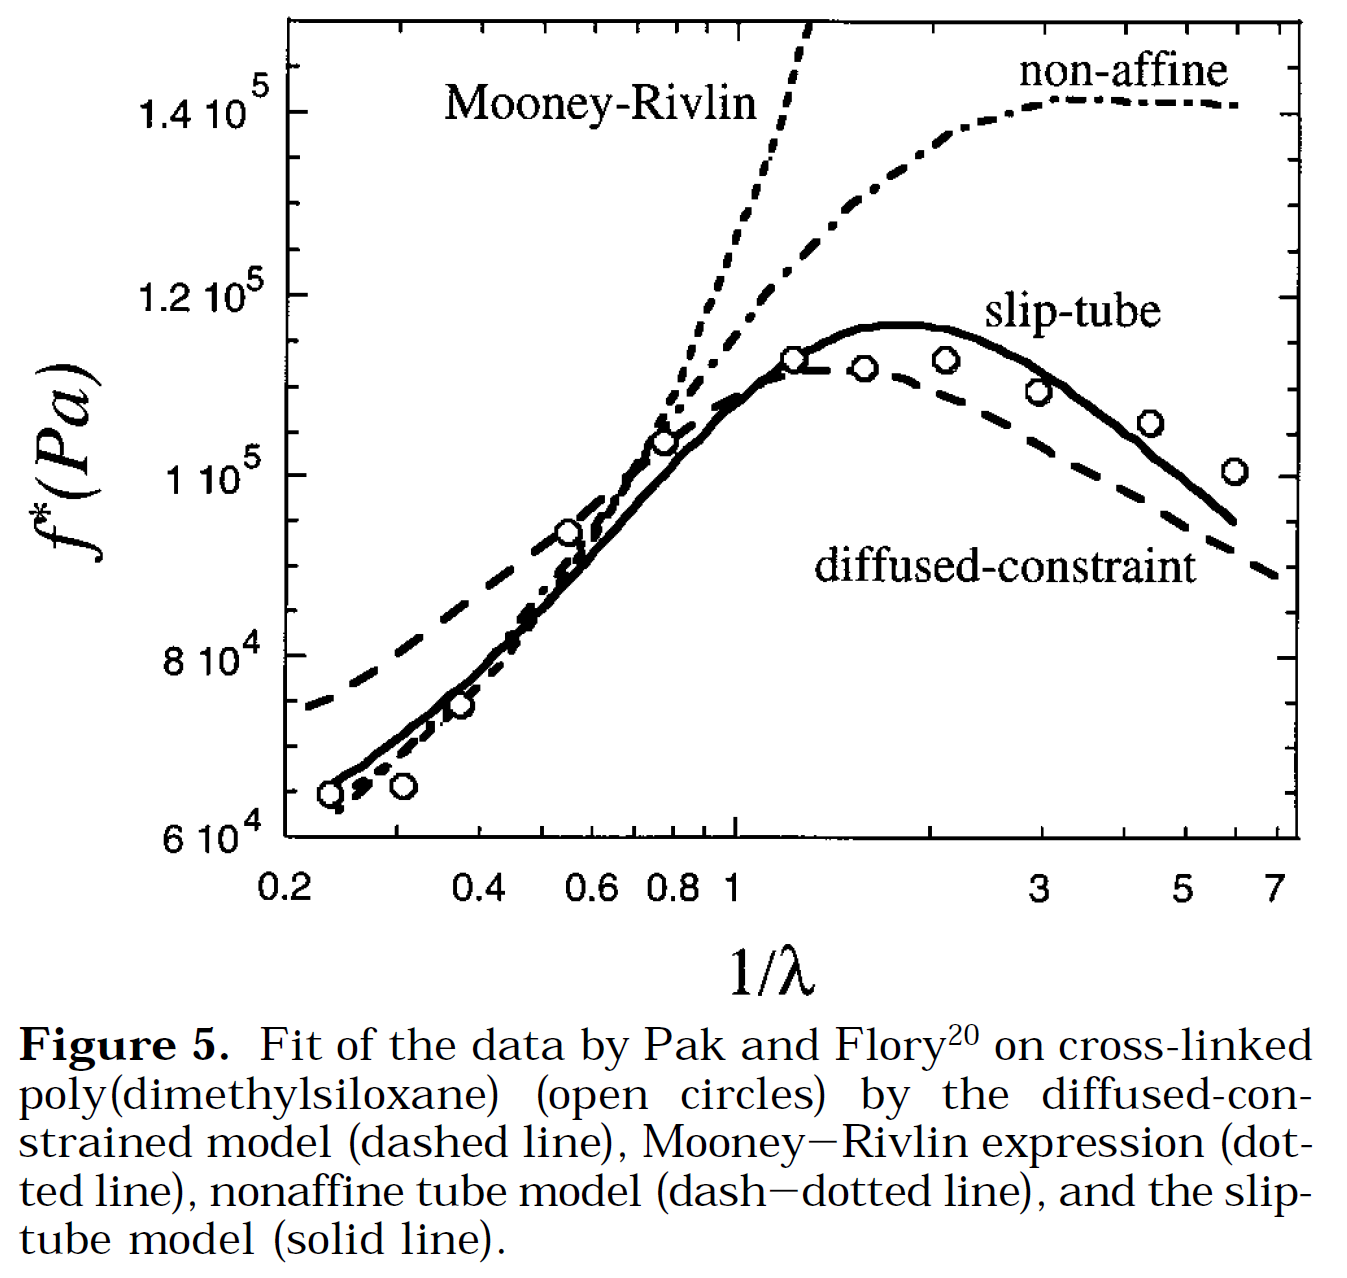
\includegraphics[width=.8\textwidth]{NW_model_rubinstein.png}
% 		\end{columns}
% \end{frame}

% \section{ランダムネットワークの検討}
% \subsection{ランダムネットワークについて}

% \begin{frame}
% 	\frametitle{規則構造からランダム構造へ}
% 		\begin{alertblock}{規則構造でのシミュレーションでは}
% 			\begin{itemize}
% 				\item アフィンネットワークモデルでの単純な緩和挙動 
% 				\begin{itemize}
% 					\item ガラス転移終端近傍に主緩和
% 					% \item ゆらぎの異方性が少ないためか?
% 				\end{itemize}
% 			\end{itemize}
% 		\end{alertblock}
% 		\begin{block}{ランダムネットワークの検討}
% 			\begin{itemize}
% 				\item ネットワーク構造の連結性に\alert{ランダム性を導入}
%                     \begin{itemize}
% 						\item \alert{Flory のファントムネットワークの要件に合致}\footnote{
% 							P. J. Flory, Proc. R. Soc. London. Series A, 351, 351 (1976)
% 						}
% 					\end{itemize}
% 				\item ランダムネットワークモデルの特徴
% 				\begin{itemize}
% 					\item アフィン変形を抑制?
% 					\item 架橋点のゆらぎに起因した多様な緩和モードが発現?
% 					\item 緩和強度の増大、あるいは、長時間化?
% 				\end{itemize}
% 			\end{itemize}
% 		\end{block}
% \end{frame}

% \begin{frame}
%     \frametitle{ランダム性の導入}
%     \vspace{-3mm}
% 		\begin{columns}[totalwidth=1\textwidth]
% 			\column{.45\textwidth}
% 				\begin{block}{連結のランダム性を導入}
% 					\begin{itemize}
% 						\item 連結性を不均一に
% 							\begin{itemize}
% 								\item 連結に\alert{位置依存性}
% 							\end{itemize}
% 						\item 巨視的な変形後
% 							\begin{itemize}
% 								\item 結節点のゆらぎが\\不均一
% 								\item 多様な緩和モード
% 								\item \alert{緩和の長時間化?}
% 							% \item ファントムネットワークモデルの諸特性の発現?
% 							\end{itemize}
% 						\item \alert{解析を容易}に、
%                             \begin{itemize}
%                                 \item 既往研究で反応系
% 								\item \alert{ストランド長と\\結合数を一定}
% 							\end{itemize}
% 					\end{itemize}
% 				\end{block}
% 			\column{.52\textwidth}
% 				ランダム構造の模式図
% 				\vspace{5mm}
% 				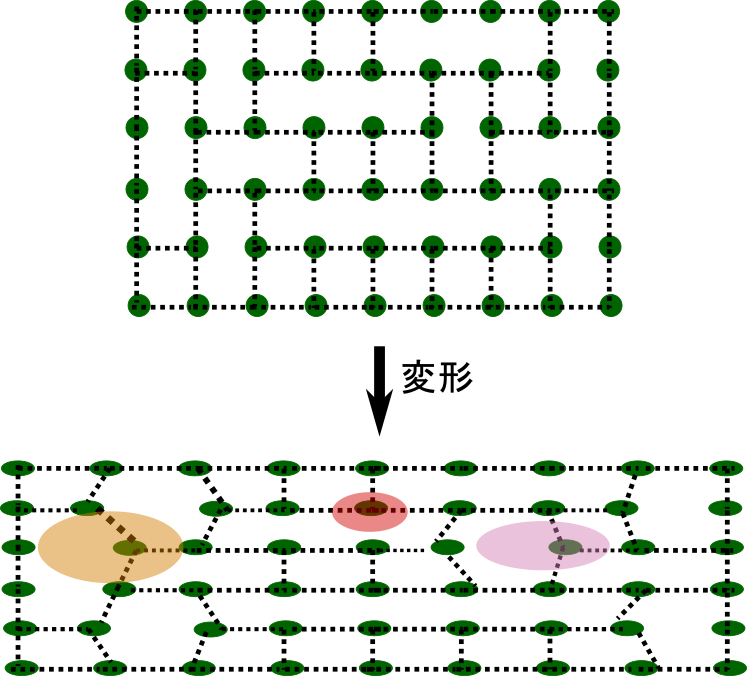
\includegraphics[width=\textwidth]{random_NW.png}
%     \end{columns}
% \end{frame}

% \subsection{ランダムネットワークの作成}
% \begin{frame}
% 	\frametitle{ランダムネットワークの作成}
% 	\vspace{-3mm}
% 	\begin{block}{初期構造の作成}
% 		\begin{enumerate}
% 			\item \alert{実空間}で8-Chain Model から初期構造を作成。
% 				\begin{itemize}
% 					\normalsize
% 					\item 所望の分岐数に\alert{ランダム}に選択した\alert{結合を除去}
% 					\item 除去したジオメトリー$\Rightarrow$\alert{トポロジーモデル}
% 				\end{itemize}
% 			\item トポロジー空間でランダム性の導入
% 				\begin{itemize}
% 					\normalsize
% 					\item \alert{エッジ交換}でノードごとにランダムな接続性導入
% 				\end{itemize}	
% 			\item 対応する\alert{実空間でのネットワーク初期構造}を作成
% 			\item \alert{適正なストランド長}となるように多重度設定
% 			\item \alert{Slow Push Offにより初期構造を緩和}
% 		\end{enumerate}

% 		\vspace{-1mm}
% 		\begin{columns}[T, onlytextwidth]
% 			\column{.33\linewidth}
% 				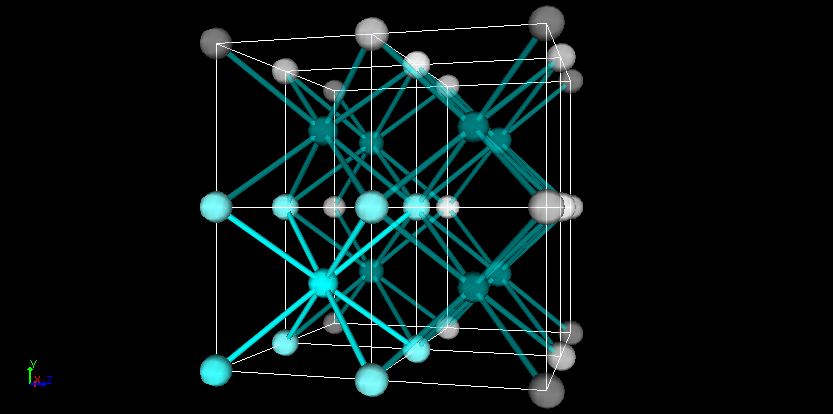
\includegraphics[width=\textwidth]{8_per.png}
% 			\column{.33\linewidth}
% 				\vspace{-5mm}
% 				\begin{center}
% 					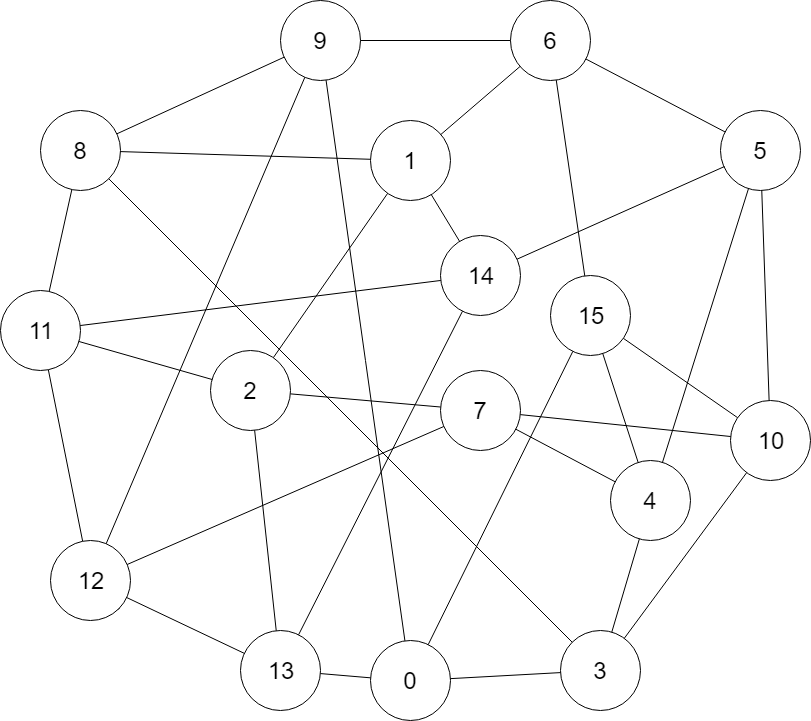
\includegraphics[width=.6\textwidth]{Network.png}
% 				\end{center}
% 			\column{.33\linewidth}
% 				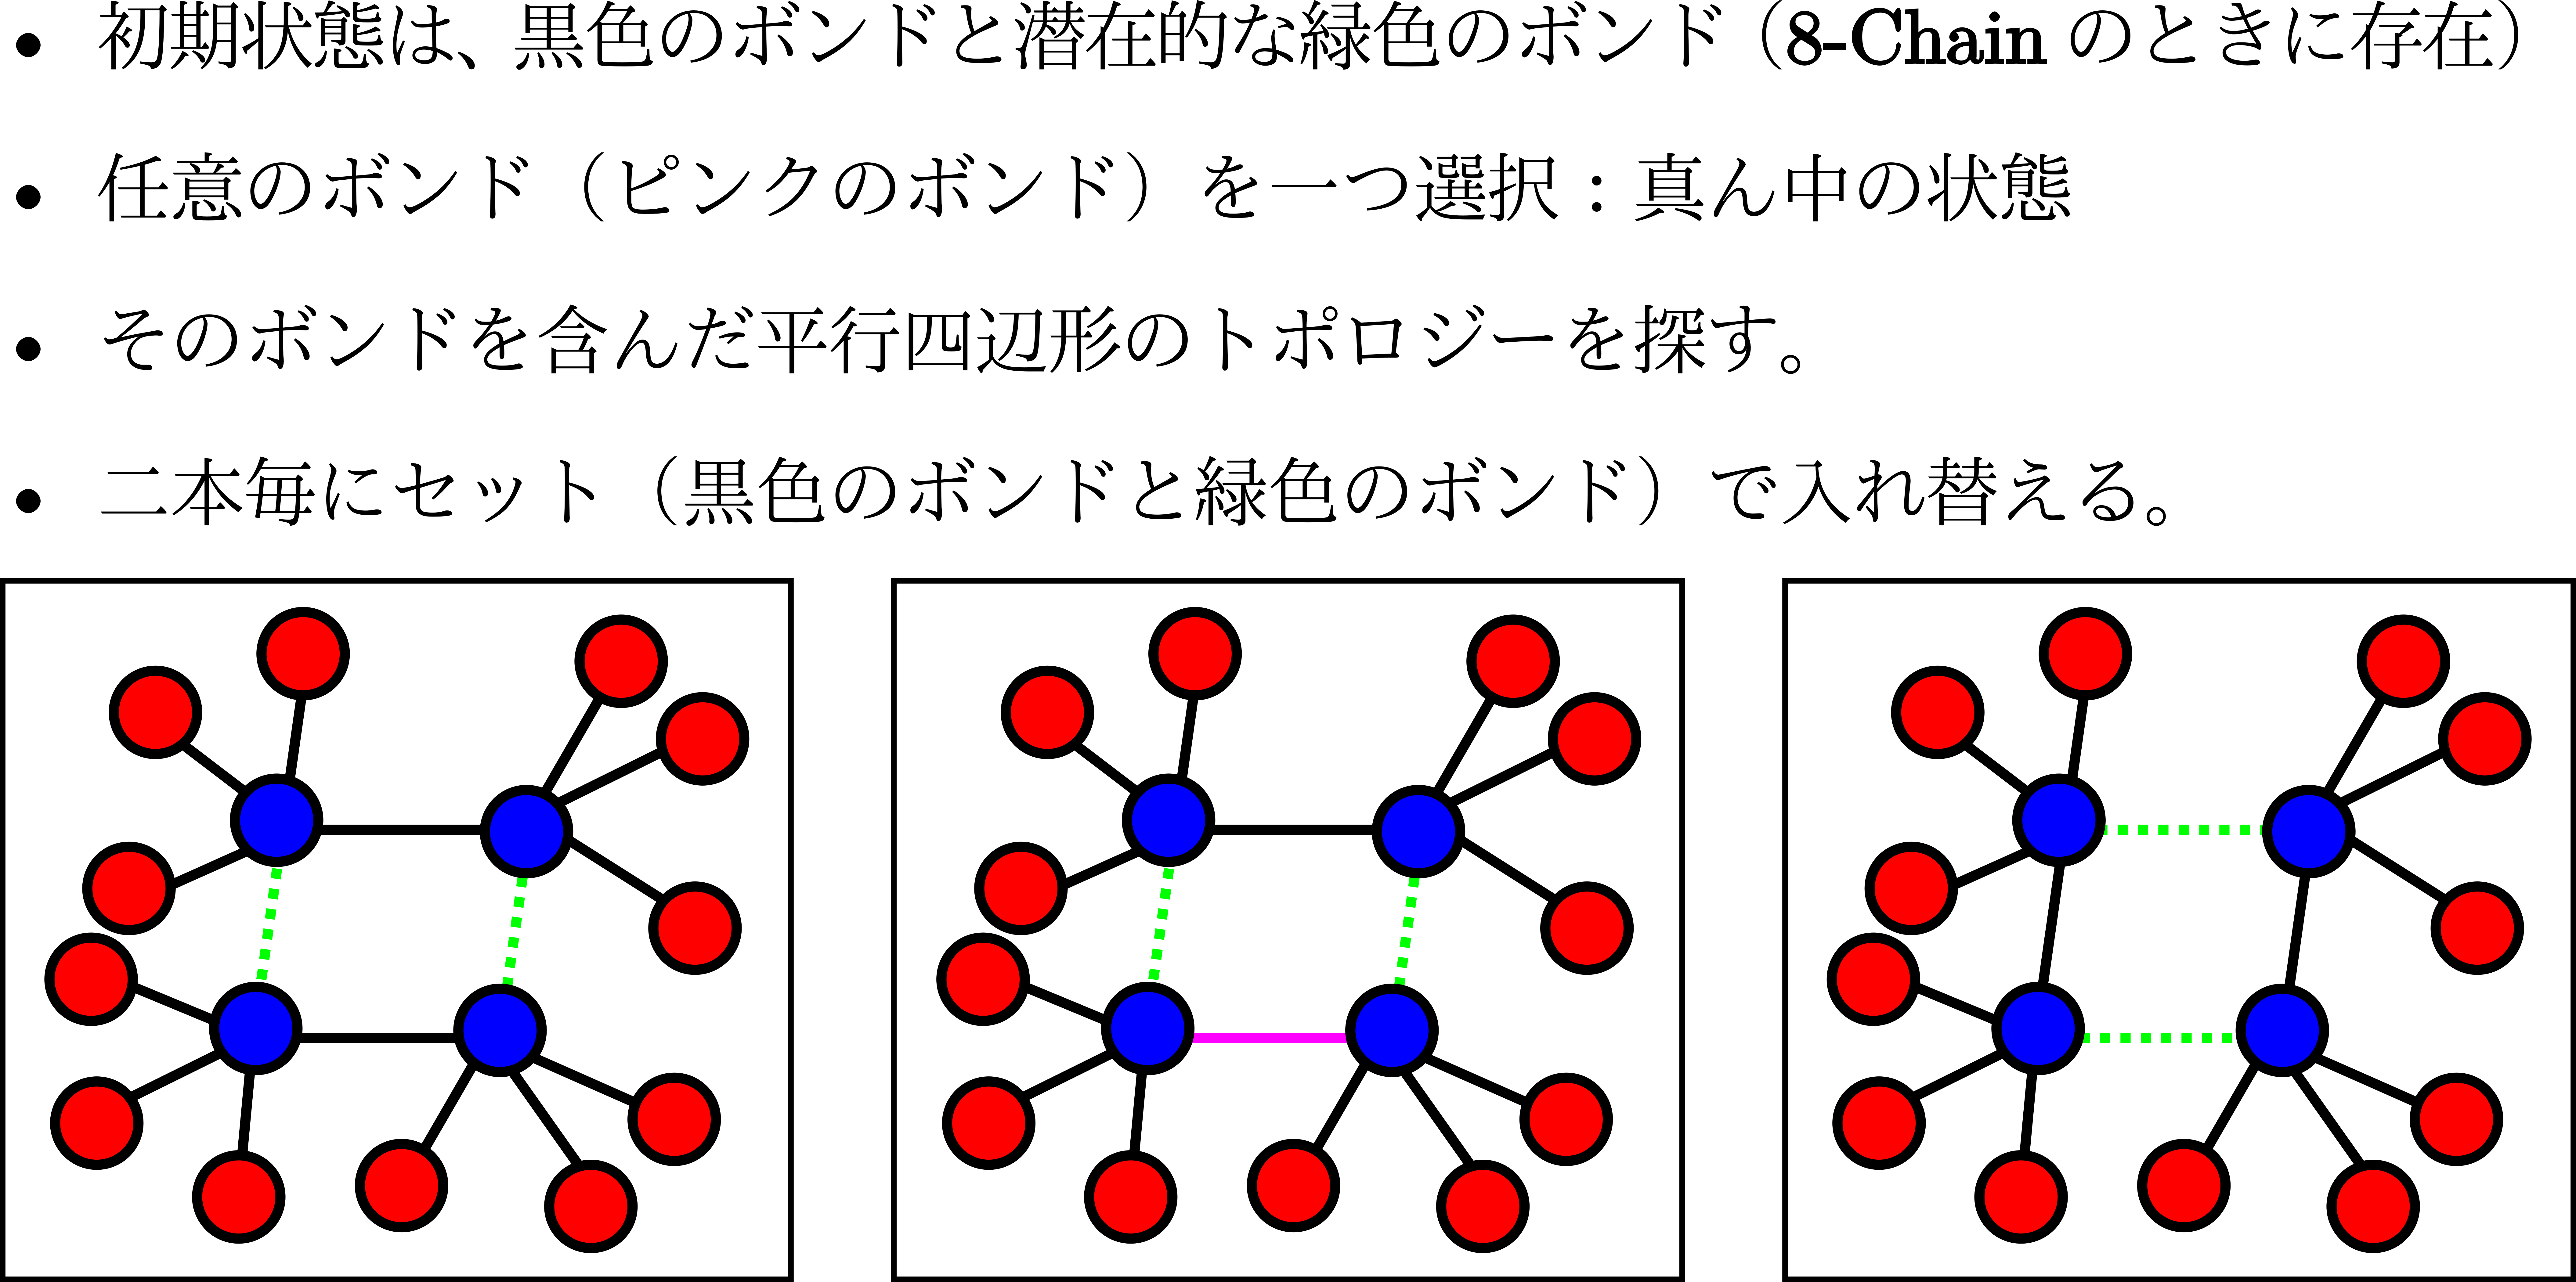
\includegraphics[width=\textwidth]{bond_exchg.png}
% 		\end{columns}
% 	\end{block}
% \end{frame}

% \begin{frame}
%     \frametitle{初期構造の緩和}
%         \vspace{-2mm}
% 		\begin{block}{KG 鎖をストランドとするネットワーク}
% 			\begin{itemize}
% 				\item KG鎖は「非素抜け」なので、\alert{初期構造の緩和}が重要。
% 					\fontsize{6pt}{0pt}
% 					\begin{align*}
% 						&U_{KG}(r) = 
% 						\begin{cases}
% 						U_{nonbond} = U_{LJ} \;\text{where } r_c = 2^{(1/6)}\sigma \\
% 						U_{bond} = U_{LJ} + U_{FENE}
% 						\end{cases} 
% 					\end{align*}
% 			\end{itemize}
% 		\end{block}
% 		\vspace{-3mm}
% 		\begin{columns}[T, onlytextwidth]
% 			\column{.66\linewidth}
% 				\begin{exampleblock}{初期構造の緩和}
% 					\begin{itemize}
% 						\item Auhl 等の方法\footnote{
% 							\scriptsize{R. Auhl et al. J. of Chem. Phys., 119, 12718 (2003)}
% 						}に従い、
% 						\begin{itemize}
% 							\item force-capped-LJ ポテンシャル
% 							\item Slow Push Off で初期構造を緩和
% 						\end{itemize}
% 					\end{itemize}
% 					\fontsize{6pt}{0pt}
% 					\begin{align*}
% 						&U_{FCLJ}(r) = 
% 						\begin{cases}
% 						(r-r_{fc})*U_{LJ}^{\prime}(r_{fc}) + U_{LJ}(r_{fc}) \; &r< r_{fc} \\
% 						U_{LJ}   \;\;\;\;\;\;\; &r \geq r_{fc}
% 						\end{cases} 
% 					\end{align*}
% 				\end{exampleblock}
% 			\column{.32\linewidth}
% 				\vspace{2mm}
% 				\begin{center}
% 					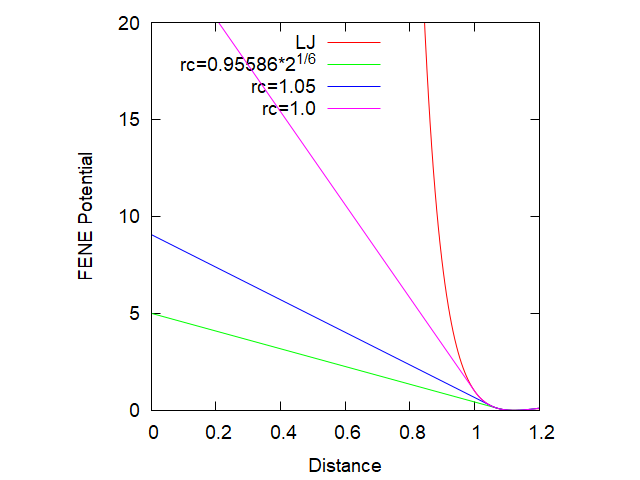
\includegraphics[width=1.2\textwidth]{Ev_fcLJ.png}
% 				\end{center}
% 				\vspace{-3mm}
% 				\scriptsize
% 				\begin{itemize}
% 					\item force-capped-LJ Pot.
% 					\item 素抜け⇒絡み合い
% 				\end{itemize}
% 		\end{columns}
% \end{frame}

% \subsection{ランダムネットワークのシミュレーション}
% \begin{frame}
% 	\frametitle{「素抜け鎖」の力学応答}
% 		\begin{alertblock}{「素抜け鎖」でのランダムネットワーク}
% 			\begin{itemize}
% 				% \item ストランド:す抜け鎖
% 				\item \alert{「排除体積効果および絡み合いのない」}ネットワーク
% 			\end{itemize}
%         \end{alertblock}
%         \vspace{-3mm}
% 		\begin{columns}[totalwidth=\linewidth]
% 			\column{.48\linewidth}
% 				\begin{block}{一軸伸張結果}
% 					\begin{itemize}
% 						\item 伸張速度低下で\\\alert{ファントム応答}に漸近
% 						% \item 低伸張率から伸び切り
%                     \end{itemize}
%                     \begin{center}
%                         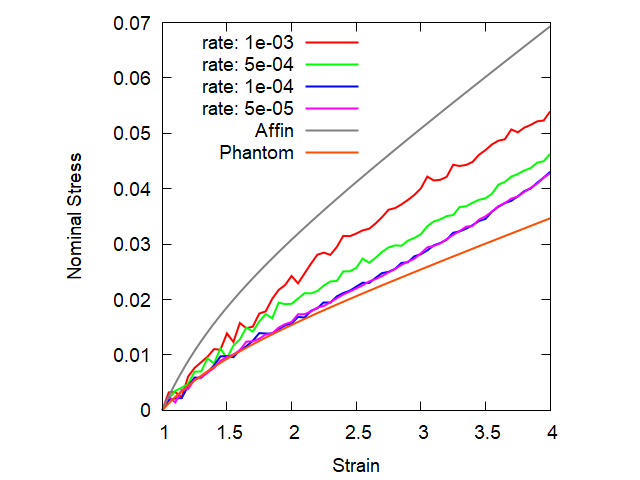
\includegraphics[width=.9\columnwidth]{N48_sunuke.png}
%                     \end{center}
% 				\end{block}
% 			\column{.48\linewidth}
% 				\begin{exampleblock}{ステップ変形の応力緩和}
%                     \begin{itemize}
%                         \item 高速伸長:$\dot{\gamma} = 1e^{-3}$
%                         \item 変位:$\lambda = 1.5$
%                     \end{itemize}
% 					\begin{center}
%                         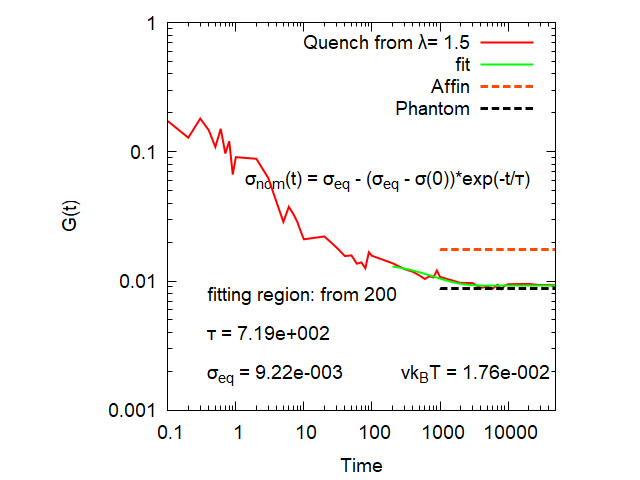
\includegraphics[width=.9\columnwidth]{gt_sunuke.png}
%                     \end{center}
% 				\end{exampleblock}
% 		\end{columns}
% \end{frame}

% \begin{frame}
% 	\frametitle{KG 鎖の力学応答}
% 	\vspace{-3mm}
% 	\begin{alertblock}{KG 鎖の四分岐ランダムネットワーク}
% 		LJ ポテンシャルによる排除体積効果および絡み合い
% 	\end{alertblock}
% 	\vspace{-4mm}
% 	\begin{columns}[T, onlytextwidth]
% 		\column{.48\linewidth}
% 			\begin{block}{一軸伸張結果}
% 				\begin{itemize}
% 					\item ネオフッキアンに漸近
% 					\item ANMよりも応力は高い
% 				\end{itemize}
% 				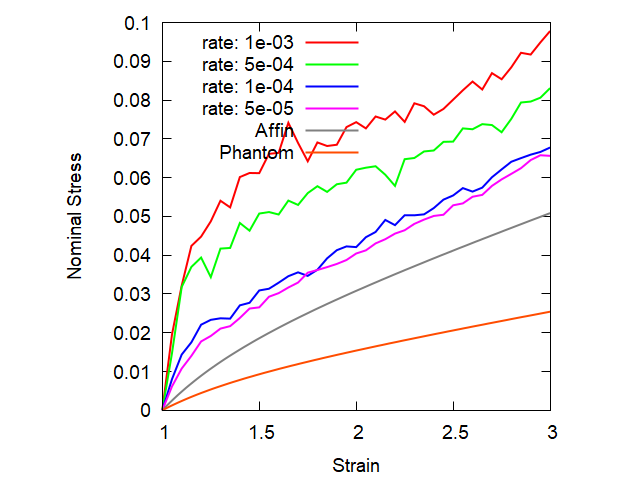
\includegraphics[width=\textwidth]{N48_C4_M3.png}
% 			\end{block}
			
% 		\column{.48\linewidth}
% 			\begin{block}{応力緩和関数 $G(t)$}
% 				\begin{itemize}
% 					\item ステップ変形($\lambda=2.0$)
% 					\item ANM よりも高弾性率
% 				\end{itemize}
% 				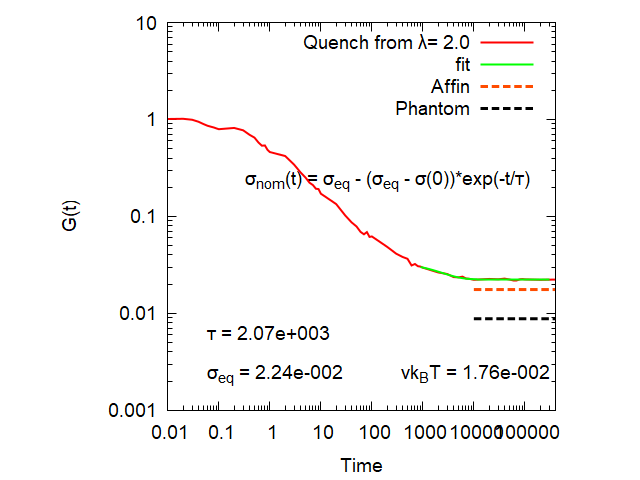
\includegraphics[width=\textwidth]{gt_N48_C4_M3.png}
% 			\end{block}
% 	\end{columns}
% \end{frame}

% \begin{frame}
%     \frametitle{ランダムネットワークの絡み合い解析: Z1-code}
%         \vspace{-2mm}
%         \begin{columns}[onlytextwidth]
%             \column{.4\linewidth}
%                 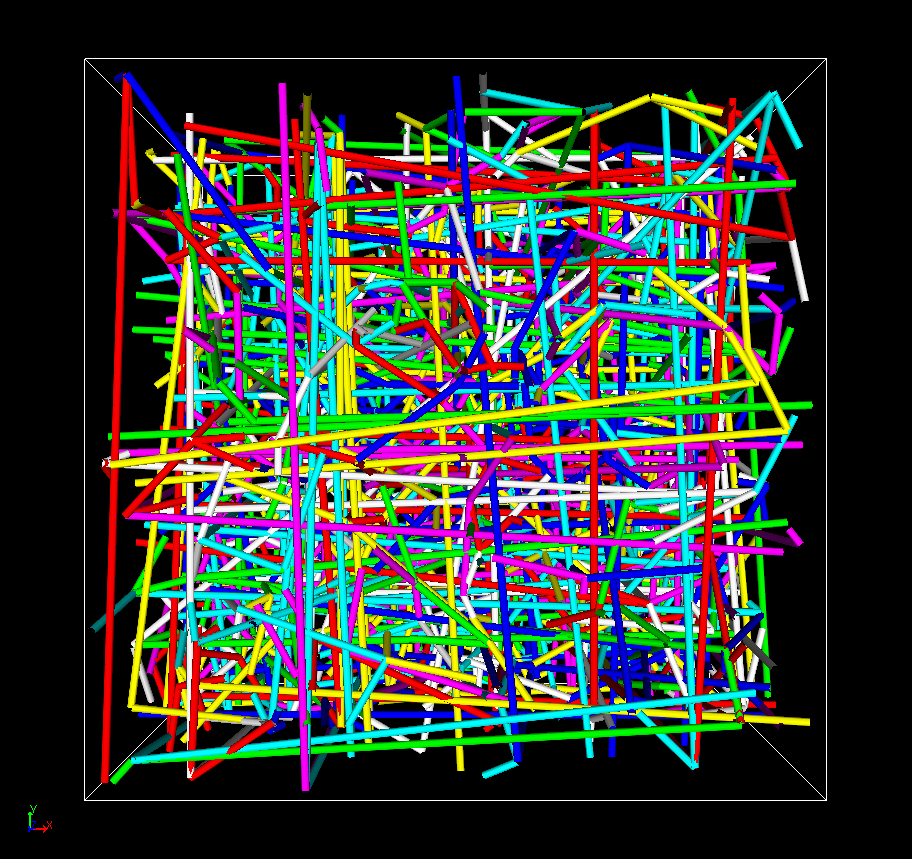
\includegraphics[width=.9\textwidth]{z_cord_4Chain.png}

%                 Z1-code での絡み合い
%             \column{.56\linewidth}
%             \begin{block}{ホモポリマーとの比較}
%                 \begin{itemize}
%                     \item Z は一本鎖あたりの絡み合い
%                     \item 今回のネットワークは、\\ホモポリマーと同等
%                 \end{itemize}
%                 \scriptsize
%                 \begin{center}
%                     \begin{tabular}{c||c|c} \hline
%                         &Homo & 4 Chain NW \\ \hline \hline
%                         Segments& 50& 48 \\ \hline
%                         Chains & 200& 768 \\ \hline
%                         Entanglements& 204& 800\\ \hline
%                         Entangled Chains&134&557 \\ \hline
%                         \alert{$<Z>_{Z1}$}&\alert{1.02}& \alert{1.04}\\ \hline
%                     \end{tabular}
%                 \end{center}
%             \end{block}
%         \end{columns}
%     \begin{alertblock}{Z1-codeとは}
%         \begin{itemize}
%             \item 絡み合いを可視化するアルゴリズム\footnote{
%                 M. Kröger, Comput. Phys. Commun. 168, 209 (2005)
%                 % \begin{itemize}
%                 %     \item M. Kröger, Comput. Phys. Commun. 168, 209 (2005)
%                 %     \item S. Shanbhag, M. Kröger, Macromolecules 40, 2897(2007)
%                 %     \item R. Hoy, K. Foteinopoulou, M. Kröger, Phys. Rev. E, 31803 (2009)
%                 % \end{itemize}
%             }
%         %    N.C. Karayiannis, M. Kröger, Int. J. Mol. Sci. 10, 5054 (2009)
%         \end{itemize}
%     \end{alertblock}
% \end{frame}

% % \begin{frame}
% %     \frametitle{絡み合いを低減したネットワーク}
% %         \vspace{-3mm}
% % 		\begin{columns}[T, onlytextwidth]
% %             \column{.45\linewidth}
% %                 \small
% % 				\begin{itemize}
% % 					\item 4-Chain-\alert{NPT}
% % 					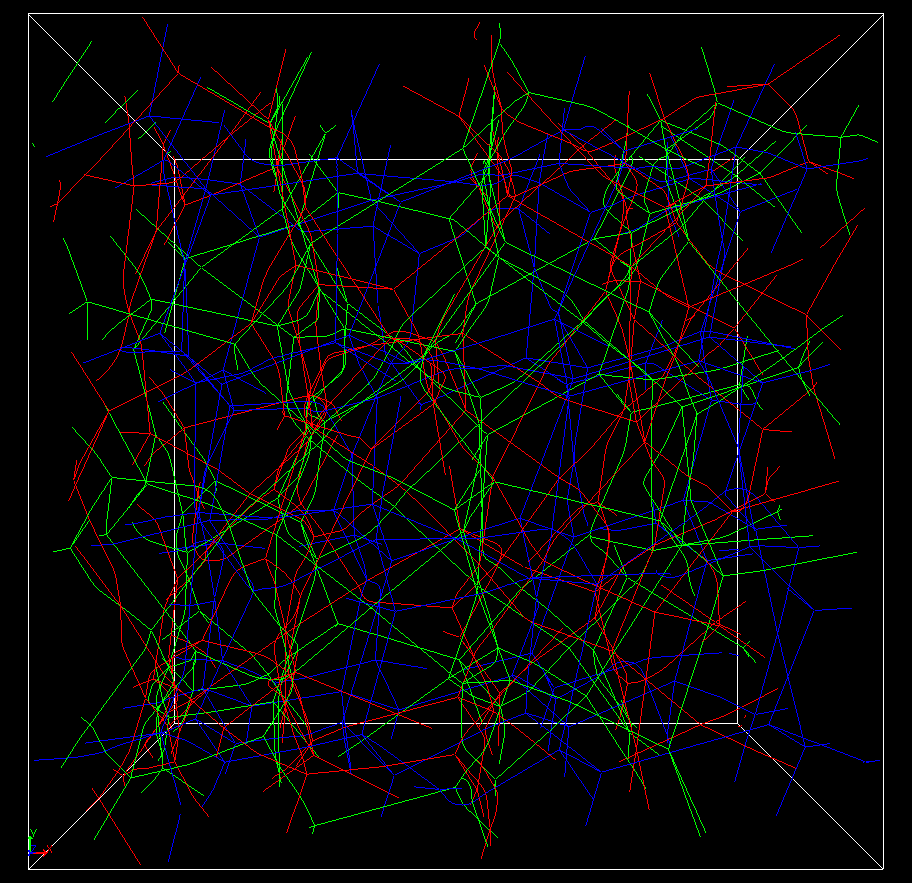
\includegraphics[width=.62\textwidth]{NPT_PPA.png}
% % 					\item 4-Chain-NVT
% % 					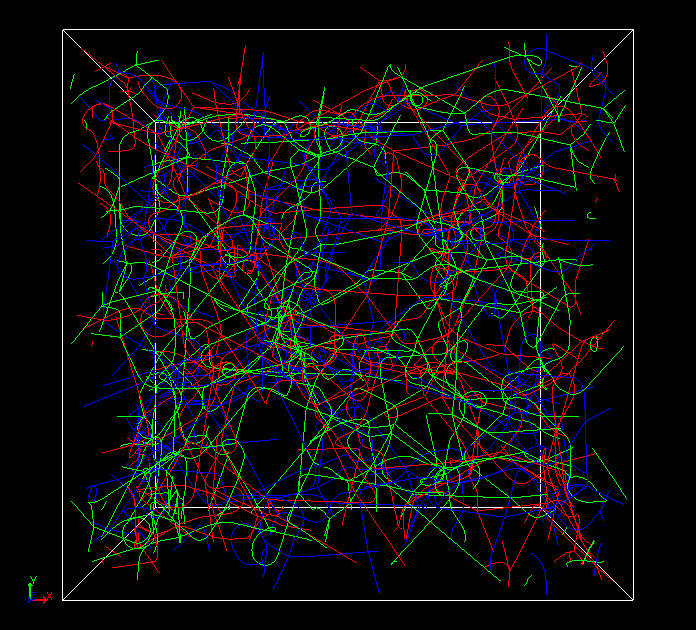
\includegraphics[width=.62\textwidth]{N48_f4_PPA.png}
% % 				\end{itemize}
% % 			\column{.55\linewidth}
% % 			\begin{block}{応力緩和関数 $G(t)$}
% % 				\begin{itemize}
% % 					\item ステップ変形($\lambda=2.0$)
% % 					\item 弾性率がPNMに漸近
% % 					% \item<2> \textcolor{blue}{定数を足せばKGと類似}
% % 				\end{itemize}
% % 					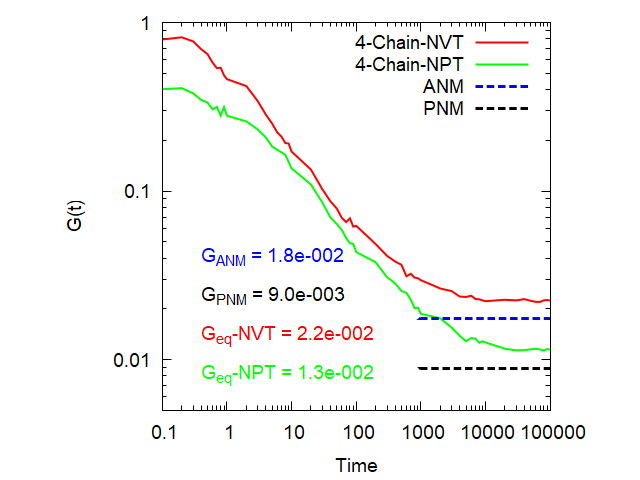
\includegraphics[width=\textwidth]{gt_4chain_comp.png}
% % 					% \includegraphics<2>[width=\textwidth]{gt_NPT_mod.png}
% % 				\end{block}
% % 		\end{columns}
% % \end{frame}

% \begin{frame}
%     \frametitle{絡み合いの効果について}
% 	\vspace{-3mm}
% 	\begin{alertblock}{絡み合い効果}
% 		% \begin{columns}[onlytextwidth]
% 		% 	\column{.8\linewidth}
% 			\small
% 			Rubinstein らの先行研究\footnote{
% 				\scriptsize{M. Rubinstein, S. Panyukov, Macromolecules, 35, 6670 (2002)}
% 				}
% 			\vspace{-3mm}
% 			\scriptsize
% 			\begin{align*}
% 				&G_c = \nu k_B T \left(1-\dfrac{2}{\phi} \right), \quad G_e = \dfrac{4}{7} \nu k_B T L \\
% 				&\text{where $\nu$ is the number density of network chains,} \\
% 				& \text{and L is the number of slip-links per network chain}
% 			\end{align*}
% 	\end{alertblock}
% 	% \vspace{-1mm}
% 	\begin{columns}[onlytextwidth]
% 		\column{.2\linewidth}
% 			\centering
% 			\vspace{3mm}
% 			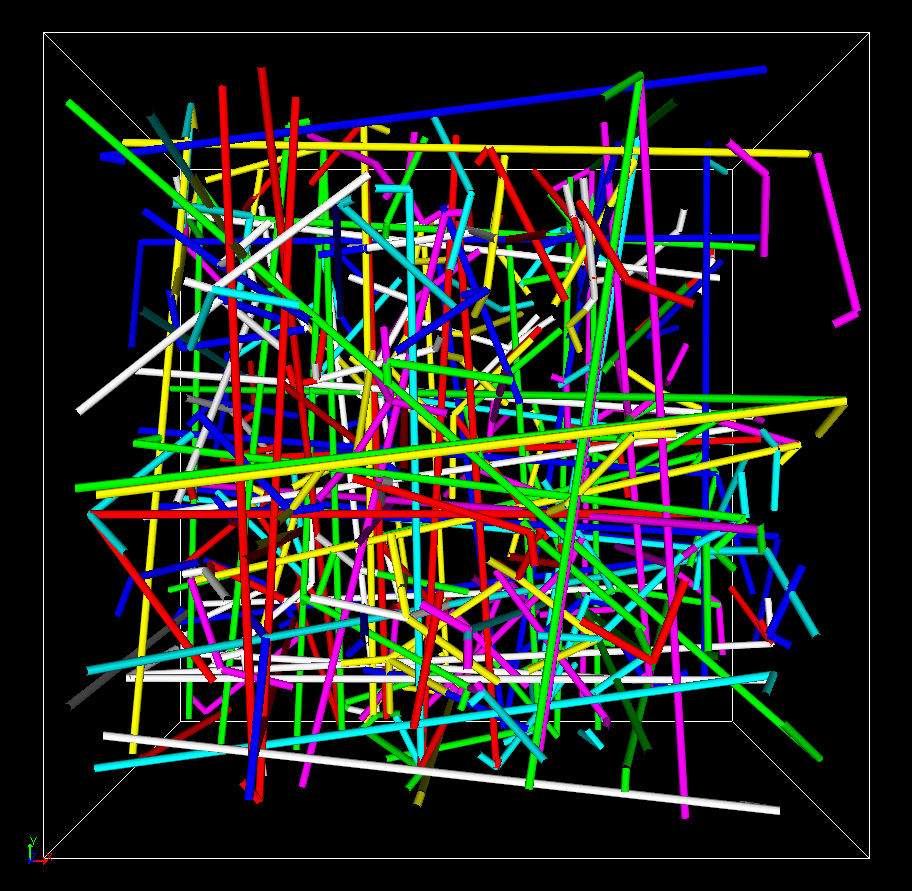
\includegraphics[width=.8\textwidth]{z_cord_NPT_4Chain.png}
% 			\vspace{2mm}
% 				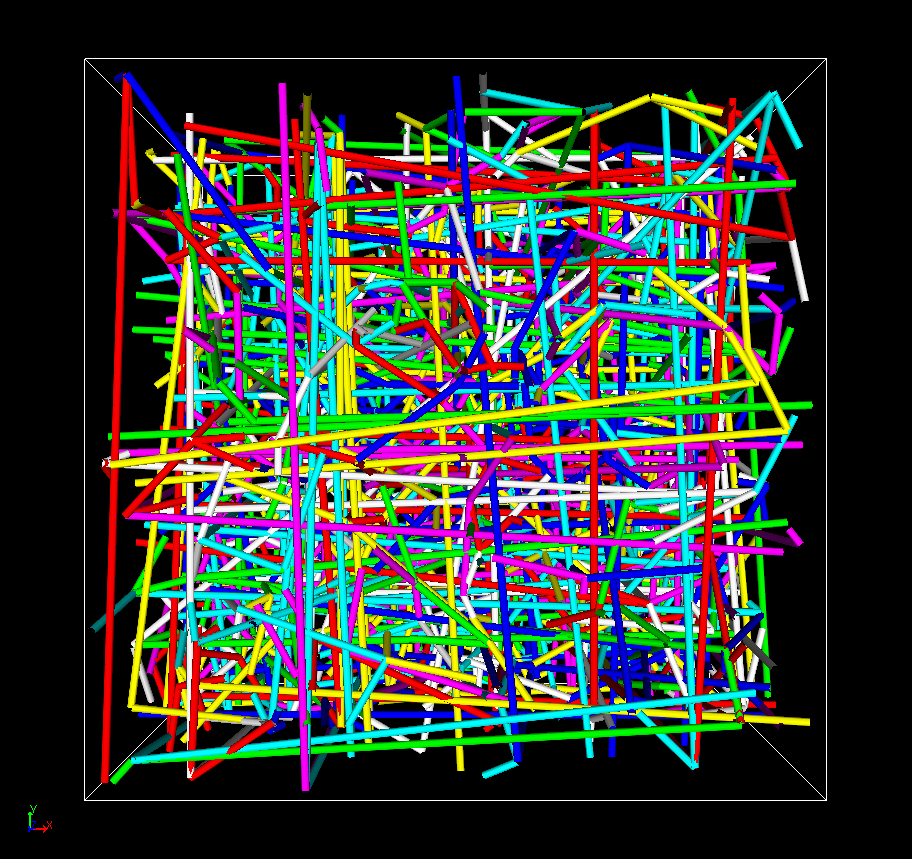
\includegraphics[width=.8\textwidth]{z_cord_4Chain.png}
% 		\column{.8\linewidth}
% 		\scriptsize
% 			\centering
% 			\begin{tabular}{c|c|c} \hline
% 				&NPT & NVT \\ \hline \hline
% 				\textcolor{blue}{Chains, $\nu$} & \multicolumn{2}{|c}{\textcolor{blue}{768, 0.018}}\\ \hline
% 				% \textcolor{blue}{$\nu$}& \multicolumn{2}{|c}{\textcolor{blue}{0.018}}\\ \hline
% 				\textcolor{blue}{$G_c = \nu \times (1-2/4)$}&\multicolumn{2}{|c}{\textcolor{blue}{0.009}} \\ \hline \hline
% 				Entanglements& 278& 800\\ \hline
% 				Entangled Chains&249&557 \\ \hline
% 				\textcolor{green}{L} & \textcolor{green}{278/768=0.36} & \textcolor{green}{800/768=1.04} \\ \hline
% 				$G_e=4/7 \times \nu \times L $ & 0.004 & 0.011 \\ \hline \hline
% 				\alert{$G_{calcd.}=G_c + G_e$} & \alert{0.013} & \alert{0.020} \\ \hline \hline
% 				$G_{measd.}$ & 0.013 & 0.022 \\ \hline
% 			\end{tabular}
% 	\end{columns}
% \end{frame}




% \section{ランダムネットワークのせん断変形}
% \subsection{分岐数の異なるネットワークのせん断変形}
% \begin{frame}
% 	\frametitle{シミュレーションによる評価}
% 	\begin{enumerate}
% 		\item 初期構造の確認
% 			\begin{itemize}
% 				\item Kr\"{o}ger らの方法により Z\_1 Code で絡み合いを評価\footnote[1]{
% 					S. Shanbhag, M. Kr\"{o}ger, Macromol. 40 2897 (2007)
% 				}
% 				\item 対応するホモポリマーメルトと同程度であることを確認
% 			\end{itemize}
% 		\item 各種アンサンブル平均を評価
% 		\item 力学特性の評価
% 			\begin{itemize}
% 				\item 一軸伸張において、生じる応力を評価
% 				\item ステップ変形による応力緩和
% 				\item \alert{Lees-Edwards 条件によりずりせん断}を付与し、生じる応力を評価
% 				\item 連続した変形を付与して、ヒステリシスを評価
% 			\end{itemize}	
% 	\end{enumerate}
% \end{frame}

% \begin{frame}
% 	\frametitle{分岐数の異なるネットワークのせん断変形}
% 	\begin{itemize}
%         \item 分岐数が異なるネットワークのせん断変形力学応答を評価した。
% 		\item 変形速度を低減することで、分岐数によらず\\Phantom Network Model:PNM へと漸近
% 	\end{itemize}

% 	\begin{columns}[T, onlytextwidth]
% 		\column{.33\linewidth}
% 			\centering
% 			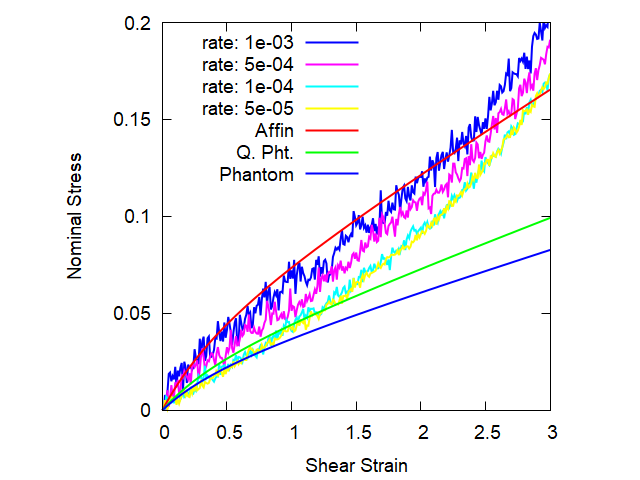
\includegraphics[width=\textwidth]{Shear_Random_4chain_N20.png}
% 			4-Chain NW
% 		\column{.33\linewidth}
% 		\centering
% 			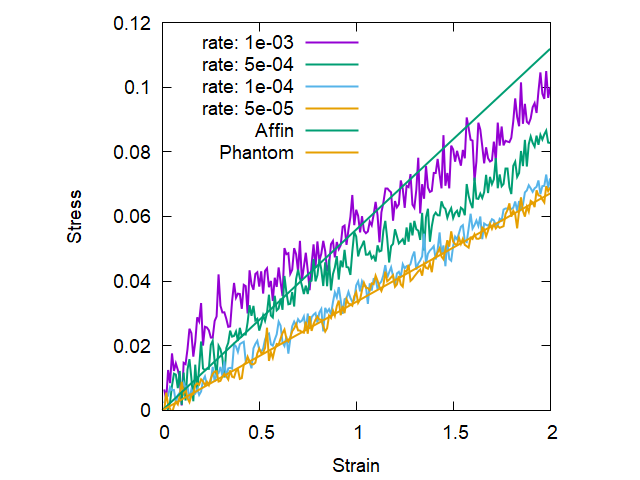
\includegraphics[width=\textwidth]{Shear_Random_5chain_N20.png}
% 			5-Chain NW
% 		\column{.33\linewidth}
% 		\centering
% 		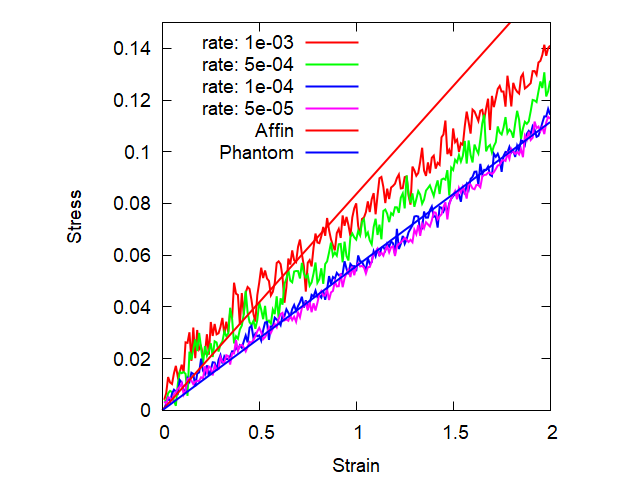
\includegraphics[width=\textwidth]{Shear_Random_6chain_N20.png}
% 		6-Chain NW
% 	\end{columns}
% \end{frame}

% \subsection{4-Cain NW のせん断変形時のヒステリシス}
% \begin{frame}
% 	\frametitle{4-Cain NW のせん断変形時のヒステリシス}
% 	\begin{itemize}
% 		% \item 変形速度の低減により、$\gamma<1$ 程度の小さなひずみでは Phantom Network Model:PNM に漸近
% 		\item PNM へと漸近する変形速度 ($\dot{\gamma} = 2e^{-4}$) で複数回の連続した変形に対しても迅速な回復を伴った力学的ヒステリシス (Hysteresis loss $\simeq$ 0.34) を示した。
% 	\end{itemize}

% 	\begin{columns}[totalwidth=\linewidth]
% 		\column{.5\textwidth}
% 			\centering
% 				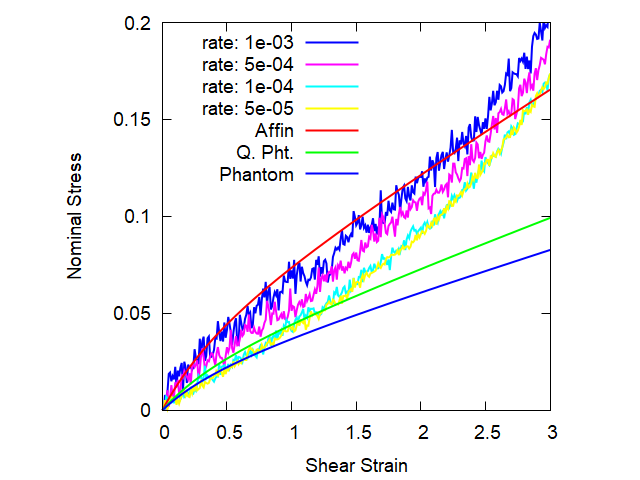
\includegraphics[width=\textwidth]{Shear_Random_4chain_N20.png}
% 				Stress-Strain Curves for 4-chain NW 
% 		\column{.5\textwidth}
% 			\centering
% 				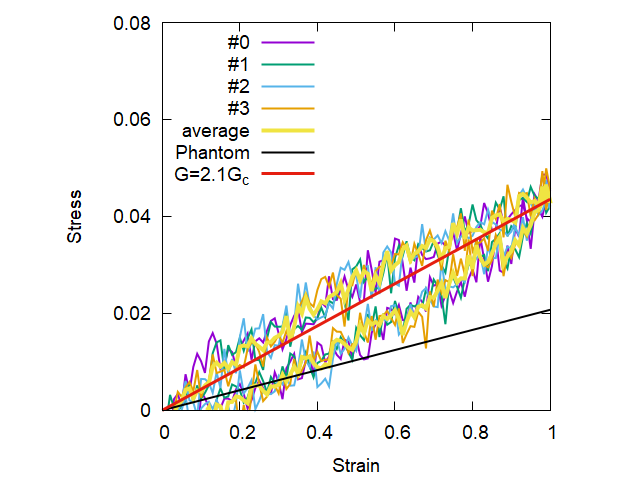
\includegraphics[width=\textwidth]{CyclicDeform_4chain_rate_2e-4.png}
% 				Hysteresis Response with Cyclic Deformations
% 		\end{columns}
% \end{frame}


% \begin{frame}
% 	\frametitle{各種の変形条件での力学的ヒステリシス}
% 		\centering
% 			\includegraphics[width=\textwidth]{hyst_shear_all.png}
% 			Hysteresis losses for valid shear rate and maximum deformation
% \end{frame}

% \begin{frame}
% 	\frametitle{ヒステリシスロス}
% 	\begin{itemize}
% 		\item 変形速度の低下に伴いヒステリシスロスは減少
% 		\item \textcolor{red}{$\dot{\gamma} \sim 1e^{-5}$ 程度のオーダーの時間スケールで消失}
% 	\end{itemize}
% 			\centering
% 				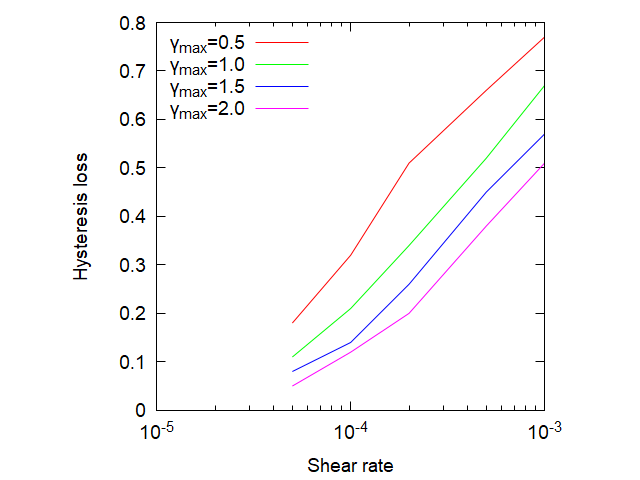
\includegraphics[width=.6\textwidth]{hyst_shear.png}\\
% 					Comparison of Hysteresis losses for 4-Chain NW
% \end{frame}

% \begin{frame}
% 	\frametitle{ラウスモードの最長緩和時間}
% 		\begin{columns}[totalwidth=\linewidth]
% 			\column{.5\textwidth}
% 			\begin{itemize}
% 				\item 最長緩和時間 ($\tau$) を評価
% 				\item ストランドのラウスモード(p=1)の自己相関関数 $C_p(t)$
% 				\begin{itemize}
% 					\item 空間的な拘束のためストランドの相関は長時間極限で一定値に収束
% 					\item その値 $C_p(\infty)$ を差し引いて評価
% 					\item \textcolor{red}{$\tau \simeq 6.5e^{4}$}
% 				\end{itemize}
% 			\end{itemize}

% 			\begin{align*}
% 				C_p(t) = \langle X_p(t)X_p(0) \rangle/\langle X_p^2 \rangle
% 			\end{align*}
			
% 			\column{.5\textwidth}
% 				\centering
% 					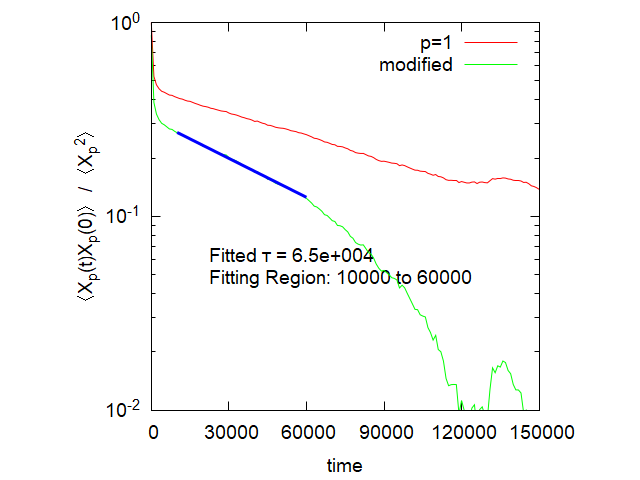
\includegraphics[width=\textwidth]{Xp_1_org.png}\\
% 					$C_{p1}(t)$ for equilibrated structure

% 			\end{columns}
% \end{frame}

% \subsection{おわりに}
% \begin{frame}
% 	\frametitle{おわりに}
% 		\begin{block}{本発表の内容}
% 			\begin{itemize}
% 				\item ストランド長が揃った分岐数の異なるランダムネットワーク
% 				\begin{itemize}
% 					\item ずりせん断での力学応答を評価
% 					\item 分岐数に応じたファントムネットワーク挙動を確認
% 				\end{itemize}
% 				\item 迅速な回復を伴った力学的ヒステリシスを確認
% 				\begin{itemize}
% 					\item ストランドの最長緩和時間が長時間化($\tau \simeq 6.5e^{4}$)
% 					\item ヒステリシスロスが消失する変形速度と対応
% 				\end{itemize}
%                 \item 今回の知見に基づき、一軸伸張での検討
% 			\end{itemize}
% 		\end{block}
% \end{frame}



% \begin{frame}
% 	\frametitle{分岐数の異なるネットワークのせん断変形}
% 	ストランド長が同一($N=20$)で分岐数のみが異なるネットワークのせん断変形力学応答を評価した。\\

% 	\begin{itemize}
% 		\item 4, 6 分岐では変形速度の低減で、分岐数によらず\\Phantom Network Model:PNM へと漸近
% 		\item 3 分岐では収束する弾性率が PNM よりも大きいものとなった
% 	\end{itemize}

% 	\begin{columns}[T, onlytextwidth]
% 		\column{.33\linewidth}
% 			\centering
% 			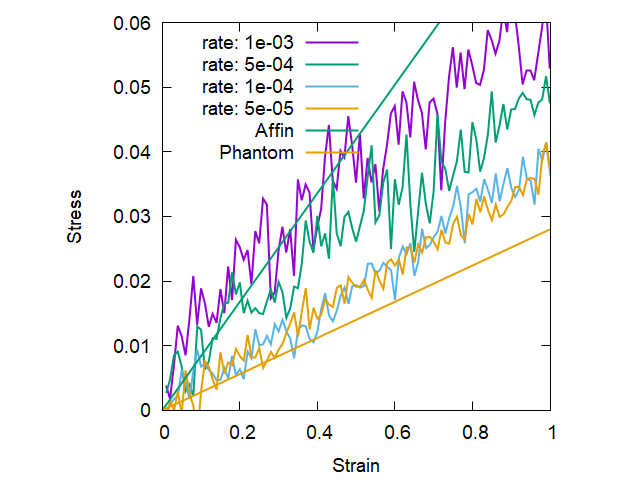
\includegraphics[width=\textwidth]{Shear_Random_3chain_N20.png}
% 			3-Chain NW
% 		\column{.33\linewidth}
% 		\centering
% 			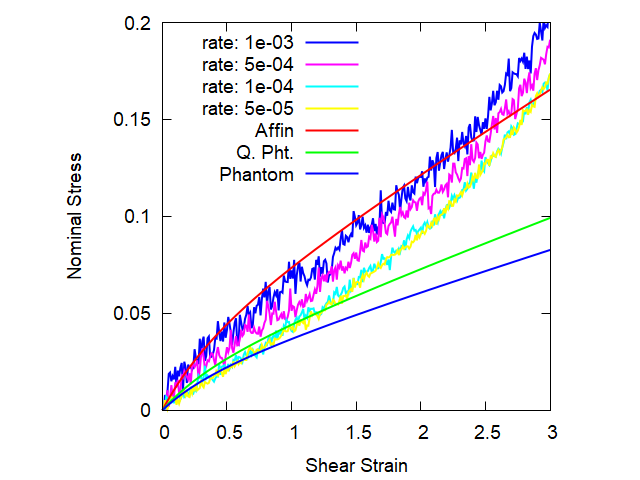
\includegraphics[width=\textwidth]{Shear_Random_4chain_N20.png}
% 			4-Chain NW
% 		\column{.33\linewidth}
% 		\centering
% 		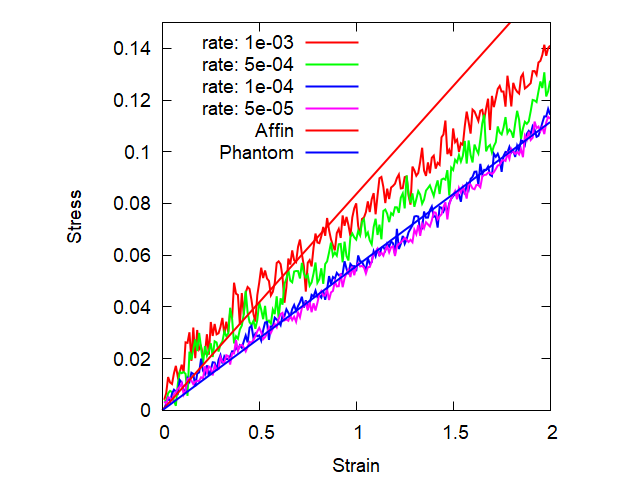
\includegraphics[width=\textwidth]{Shear_Random_6chain_N20.png}
% 		6-Chain NW
% 	\end{columns}
% \end{frame}

% %%%%%%%%%%%%%%%%%%%%%%%%%%%%%%%%%%%%%%%%%%%%%%%
% \appendix

% \backupbegin

% \begin{frame}
% 	\LARGE{補足資料}
% \end{frame}
% %%%%%%%%%%%%%%%

% \section{背景}

% \subsection{背景}

% \begin{frame}
% 	\frametitle{高分子材料への期待と不安}
% 	地球温暖化対策の CO$_2$ 削減へ向けて、\\
% 	「自動車を中心とした運送機器の抜本的な軽量化」が提唱
% 	\begin{block}{高分子材料への期待}
% 		\begin{itemize}
% 			\item 鉄鋼主体$ \Rightarrow$ \textcolor{green}{高分子材料を含むマルチマテリアル化}
% 			\item 高分子材料によるマルチマテリアル化のポイント
% 				\begin{itemize}
% 					\item \alert{高い比強度}の有効利用
% 					\item 特徴を生かした適材適所 $\Leftrightarrow$ 適切な接合方法の選択
% 						\begin{itemize}
% 							\item {\color{red} 「接着接合」}への高分子の利用
% 							\item {\color{red} 「柔らかさを生かした弾性接着接合」}
% 						\end{itemize}
% 				\end{itemize}
% 		\end{itemize}
% 	\end{block}
% 	\begin{alertblock}{柔軟材料としてゴム材料に注目}
% 		\begin{itemize}
% 			\item しなやかな強さを有する材料
% 			\item {\color{blue}強度や耐久性の定義が不明確(特に疲労破壊に対して)}
% 		\end{itemize}
% 	\end{alertblock}
% \end{frame}

% \subsection{ゴムの破壊について}

% \begin{frame}
% 	\frametitle{ガラス状態の高分子材料の疲労と破壊}
% 		\begin{columns}[totalwidth=1\textwidth]
% 			\column{.52\textwidth}
% 				\begin{block}{破壊のモード(巨視的)}
% 					脆性破壊 $\Leftrightarrow$ 延性破壊\\
% 					脆性破壊は、降伏前にミクロな\\クラックが進展した破壊
% 				\end{block}
% 			\column{.42\textwidth}
% 				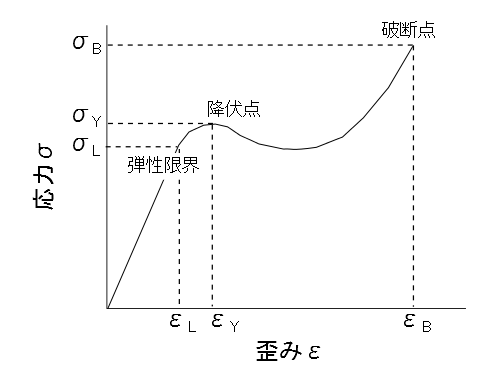
\includegraphics[width=.8\textwidth]{S_S_Curve.png}
% 		\end{columns}
% 		\begin{exampleblock}{降伏と劣化}
% 			\begin{itemize}
% 				\item 靭性向上のため
% 				\begin{itemize}
% 					\item {\color{red} 局所的な降伏}が必須。\\(クレイズのような局所的な破壊も)
% 					\item 一般に、高分子材料の{\color{red} 降伏は不可逆}。
% 				\end{itemize}
% 				\item 降伏による劣化
% 					\begin{itemize}
% 						\item 降伏 $\Leftrightarrow$ {\color{red} 本質的には、少しずつ破壊。}
% 						\item {\color{red} 破壊領域への水分の浸透 $\Leftarrow$ 長期耐久性の欠如}
% 					\end{itemize}
% 			\end{itemize}
% 		\end{exampleblock}
% \end{frame}

% \begin{frame}
%     \frametitle{破壊工学の考え方}
% 	\vspace{-2mm}
%     \begin{exampleblock}{破壊工学の考え方}
% 		\begin{itemize}
% 			\item 系中に\alert{クラックが存在することを前提}
% 			\begin{itemize}
% 				\item グリフィスの条件(脆性材料)\footnote[1]{
% 					A. A. Griffith, Phil. Trans. Roy. Soc. London, A221, 163 (1921)
% 					}
% 					\item 弾塑性材料の延性破壊への拡張\footnote[2]{
% 						G.R.Irwin, J. Appl. Mech., 24, 361 (1957)
% 						}
% 			\end{itemize}
% 		\end{itemize}
% 	\end{exampleblock}
% 	\vspace{-2mm}
% 	\begin{columns}
% 		\column{.58\textwidth}
% 			\begin{itemize}
% 				\item
% 				応力拡大係数 $K_I$ で評価
% 				\footnotesize
% 				\begin{align*}
% 				K_{I} = \sigma \sqrt{\pi c}
% 				\end{align*}
% 				\normalsize
% 				\item 
% 				先端での局所降伏領域: d\\
% 				$\Rightarrow$ 降伏応力 $\sigma_Y$ に反比例
% 				\footnotesize
% 				\begin{align*}
% 				d \propto \left( \dfrac{K_I}{\sigma_Y} \right)^2
% 				\end{align*}
% 				\normalsize
% 			\end{itemize}
% 		\column{.4\textwidth}
% 			\centering
% 			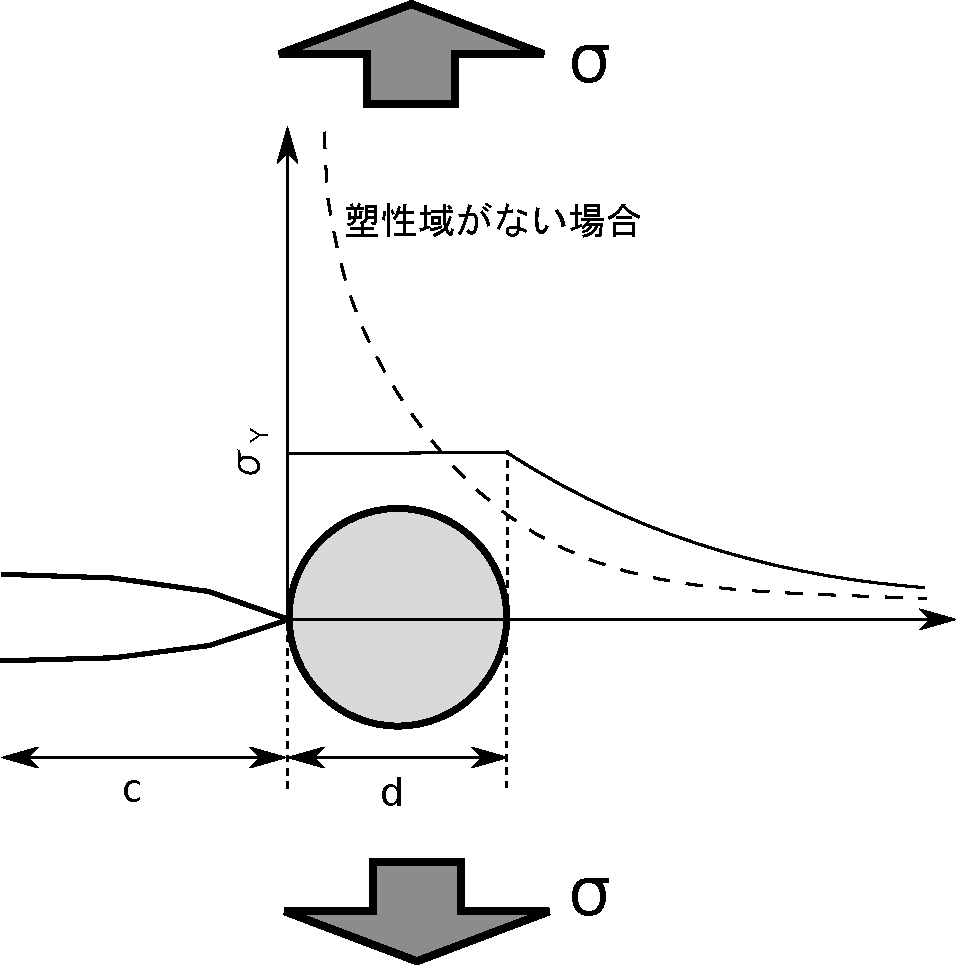
\includegraphics[width=.82\textwidth]{./Crack_Yield.pdf}
% 		\end{columns}
% \end{frame}

% \begin{frame}
% 	\frametitle{ゴムの破壊と時間温度換算則}
% 		\begin{alertblock}{ゴムの破壊について}
% 			クラック先端での大変形を伴う非線形現象だが、\\時間温度換算則の成立が多数報告\footnote{
% 				Smith T., Stedry P., J. Appl. Phys., 31 1892 (1960)
% 			}
% 		\end{alertblock}
% 		\vspace{-2mm}
% 		\begin{columns}[T, totalwidth=\textwidth]
% 			\column{.48\textwidth}
% 				亀裂先端近傍での大変形
% 				\vspace{-3mm}
% 				\begin{center}
% 					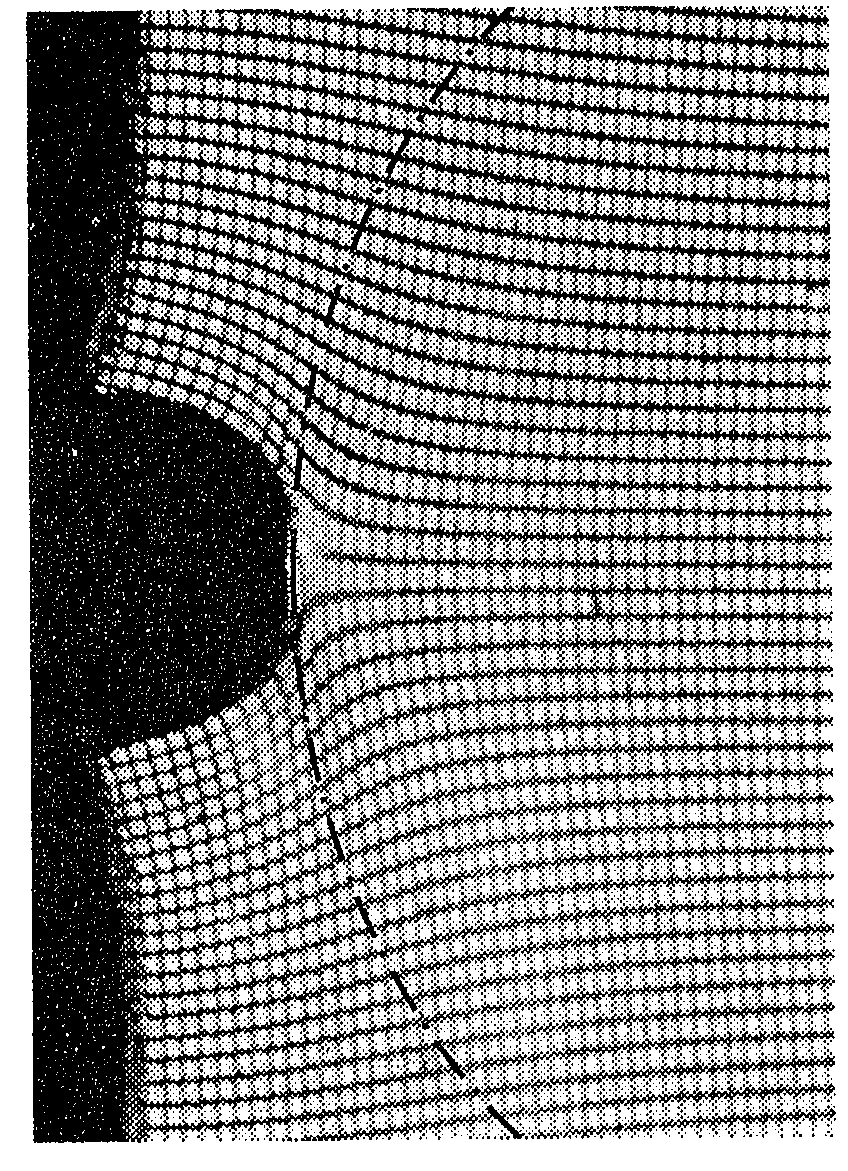
\includegraphics[width=.55\textwidth]{rubber_crack.png}
% 				\end{center}
% 			\column{.48\textwidth}
% 				時間温度換算則の成立
% 				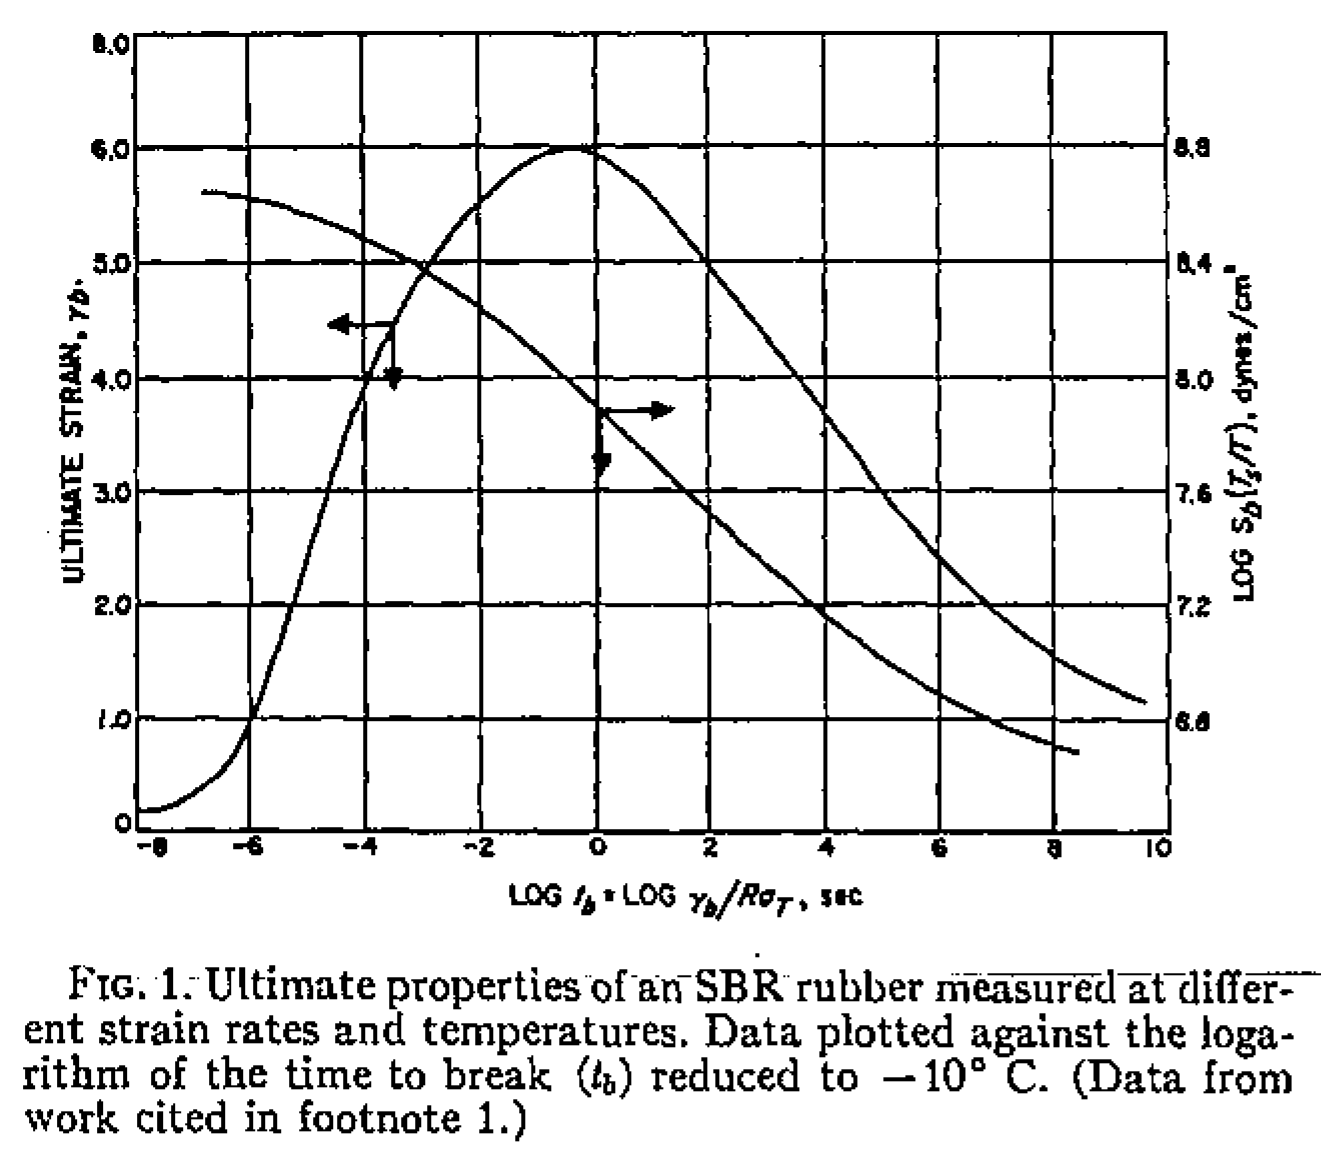
\includegraphics[width=.8\textwidth]{Time_Temp_2.png}
% 		\end{columns}
% \end{frame}

% \begin{frame}
% 	\frametitle{SBRでの伸びきり効果}
% 		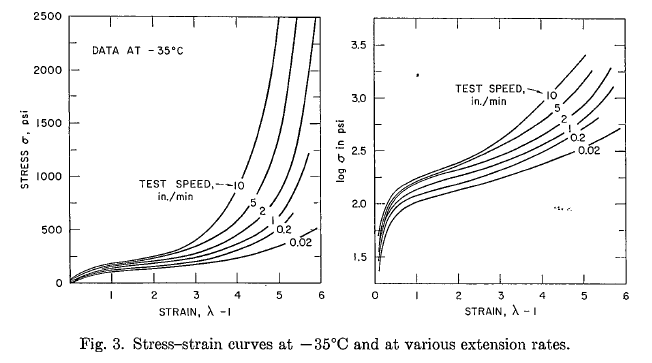
\includegraphics[width=.8\textwidth]{SBR_lowTemp_2.png}

% 		{\footnotesize Smith TL., Dickie RA., J. Pol. Sci. part A-2 (1969) 7 635}
% 		\begin{alertblock}{室温で伸び切りが出ないはずのSBR}
% 			\begin{itemize}
% 				\item 低温、高速変形でSBRでも伸びきり効果が発現
% 				\item 時間温度換算則で考えてみれば?
% 			\end{itemize}
% 		\end{alertblock}
% \end{frame}

% \begin{frame}
%     \frametitle{ゴムの破断強度の時間温度依存}
% 	\vspace{-2mm}
%     \begin{columns}[T, totalwidth=\textwidth]
%     \column{.53\textwidth}
%     \begin{itemize}
% 		\item \alert{粘弾性極限において\footnote[1]{
% 			G.J. Lake and A.G. Thomas, \\R. Soc. Lond. A300, 108 (1967)
% 		}}\\
% 		(高温・低速)
% 	\end{itemize}
%     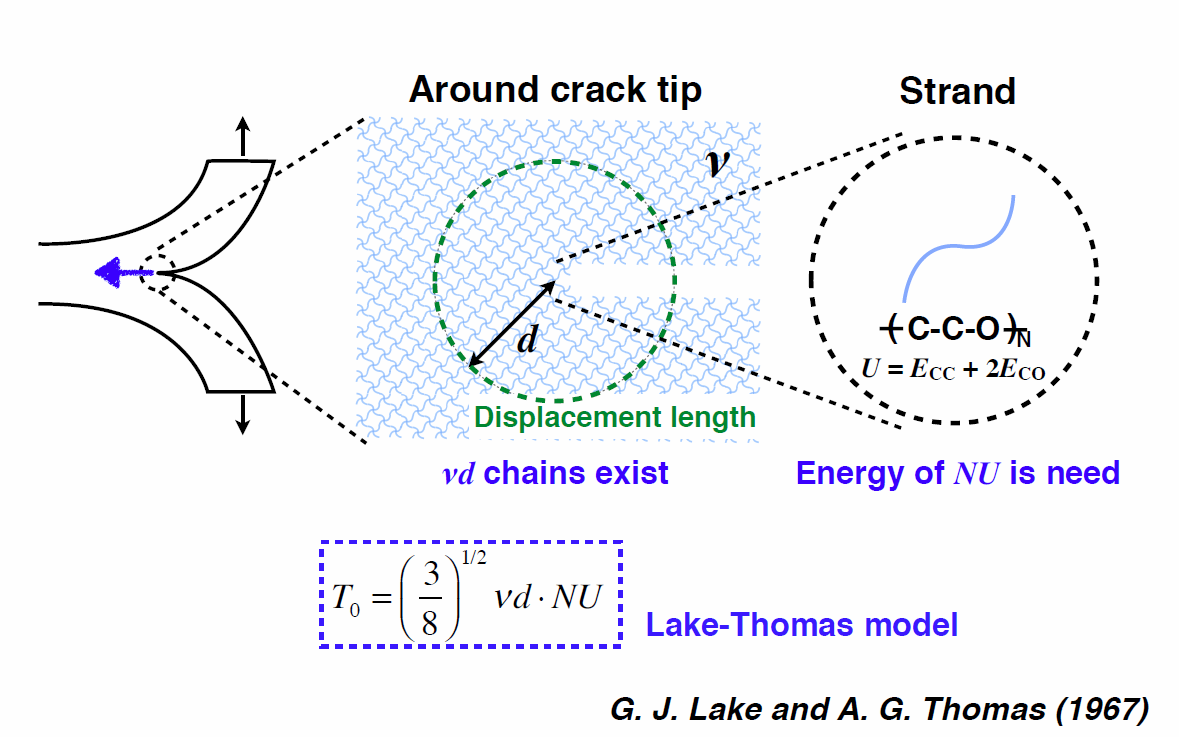
\includegraphics[width=\textwidth]{Lake_Thomas.png}
    
%     \column{.45\textwidth}
%     \begin{itemize}
% 		\item 変形速度、温度に依存\\
% 		\alert{破壊包絡線\footnote[2]{
% 			Smith T., Stedry P., \\J. Appl. Phys. (1960) 31 1892
% 		}}
% 	\end{itemize}
% 	\begin{center}
% 		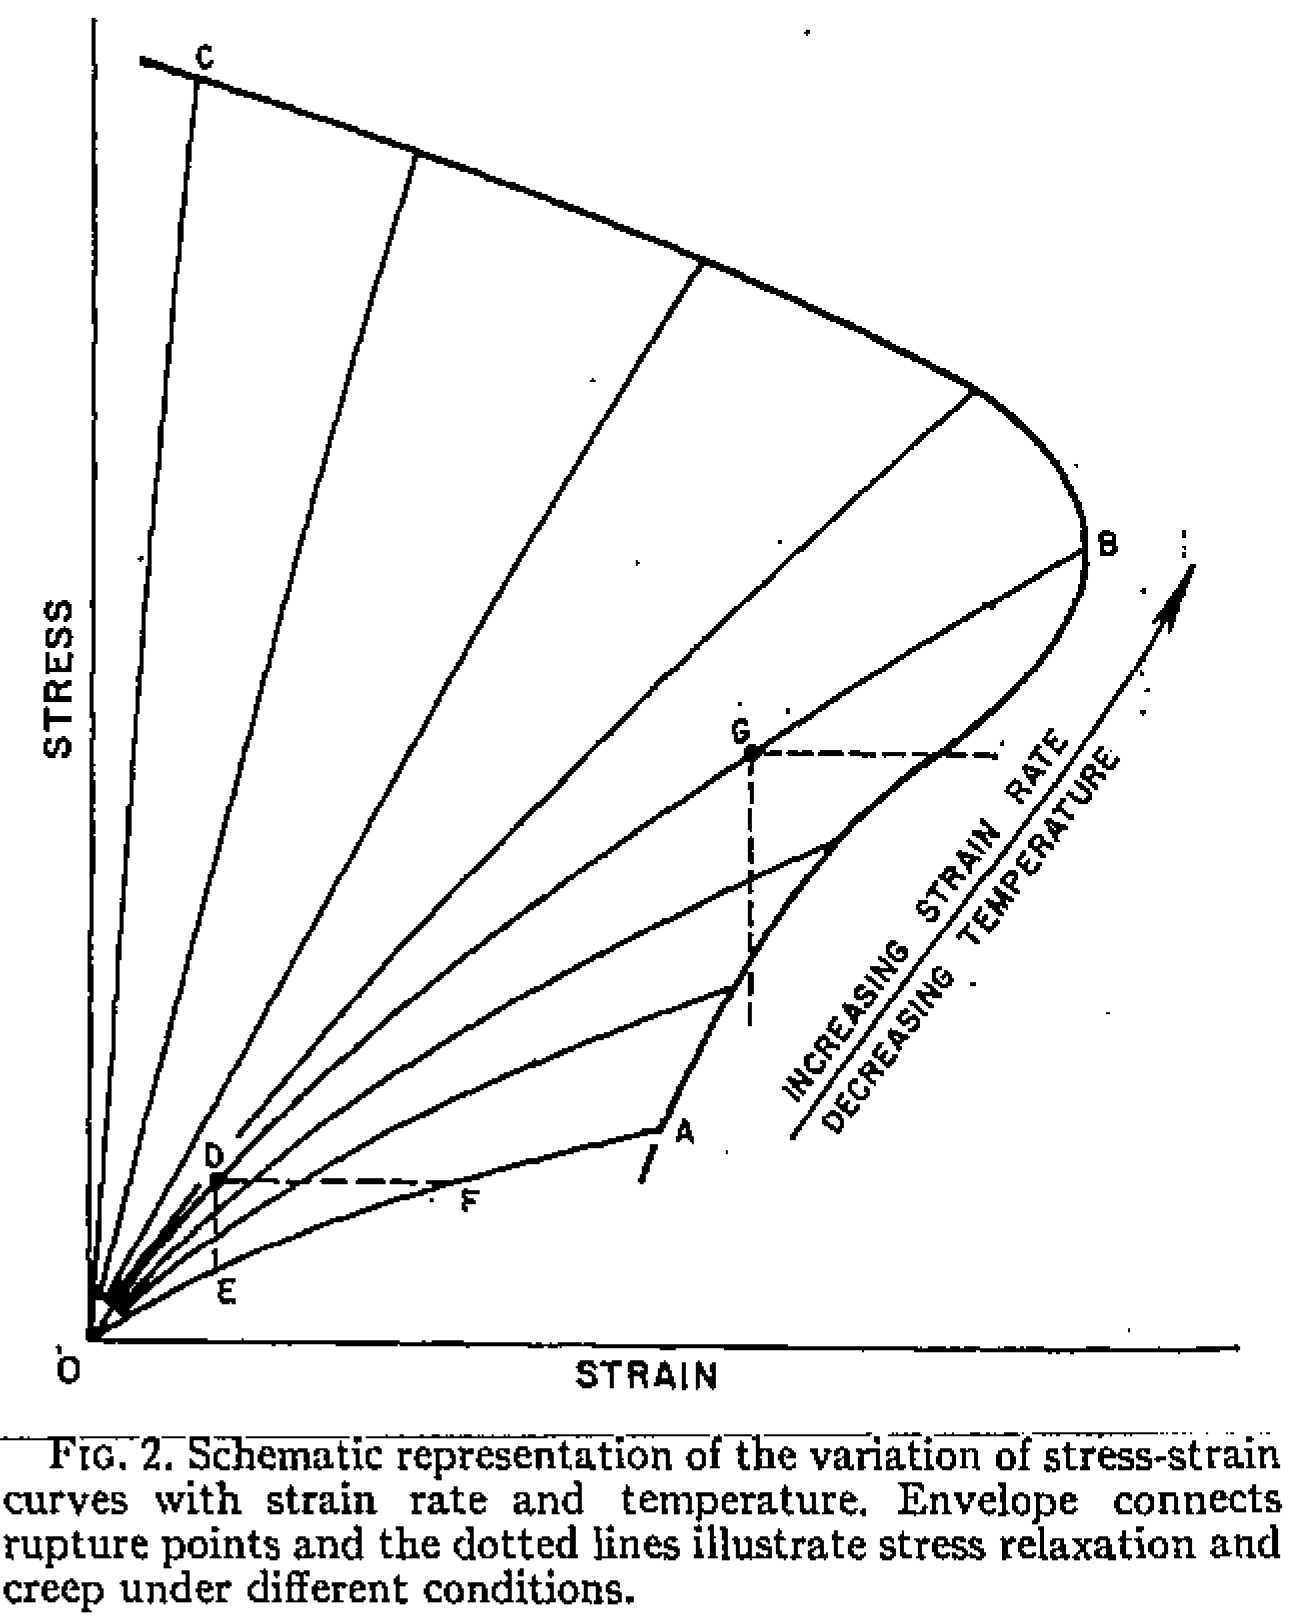
\includegraphics[width=.4\textwidth]{Time_Temp_3.png}
% 	\end{center}
%     \end{columns}
%     \begin{alertblock}{ゴムの引き裂きエネルギー}
% 		\vspace{-2mm}
% 		\begin{align*}
% 			&\mathcal{T}=\mathcal{T}_0 \times {\color{red}\Phi}(\dot{c}, T, \epsilon_0) \\
% 			&\text{where $\dot{c}$ is crack velocity and $\epsilon_0$ is applied strain}
% 		\end{align*}
%     % $\mathcal{T}=\mathcal{T}_0 \Phi(\dot{c}, T, \epsilon_0)$
%     \end{alertblock}
% \end{frame}


% \begin{frame}
% 	\frametitle{Andrews 理論}
% 	\vspace{-2mm}
% 	\begin{exampleblock}{Andrews 理論}
% 		\begin{columns}[totalwidth=1\textwidth]
% 			\column{.68\textwidth}
% 			\begin{itemize}
% 			\item クラック近傍の応力場\footnote{
% 					Andrews, E. H. and Fukahori, Y., \\J. of Mat. Sci., 12, 1307 (1977)
% 					}
% 					\begin{itemize}
% 						\item \textcolor{blue}{Loading 場}と\textcolor{red}{Unloading 場}
% 						\item クラック進展時に遷移
% 					\end{itemize}
% 			\item ヒステリシスロスを有する材料では
% 				\begin{itemize}
% 				\item
% 				\alert{この差}が、全体の変形に要した\\エネルギーの多くを\alert{散逸}
% 				\item
% 			鎖の破断へのエネルギーが低減 \\$\Rightarrow$ \alert{強靭さの起源。}
% 				\end{itemize}	
% 			\item \textcolor{green}{実験的に、$\Phi$ を求めている。}
% 			% \item \alert{ミクロな緩和現象}がマクロな耐久性向上と繋がる?
% 			\end{itemize}
		
% 			\column{.3\textwidth}
% 			\centering
% 			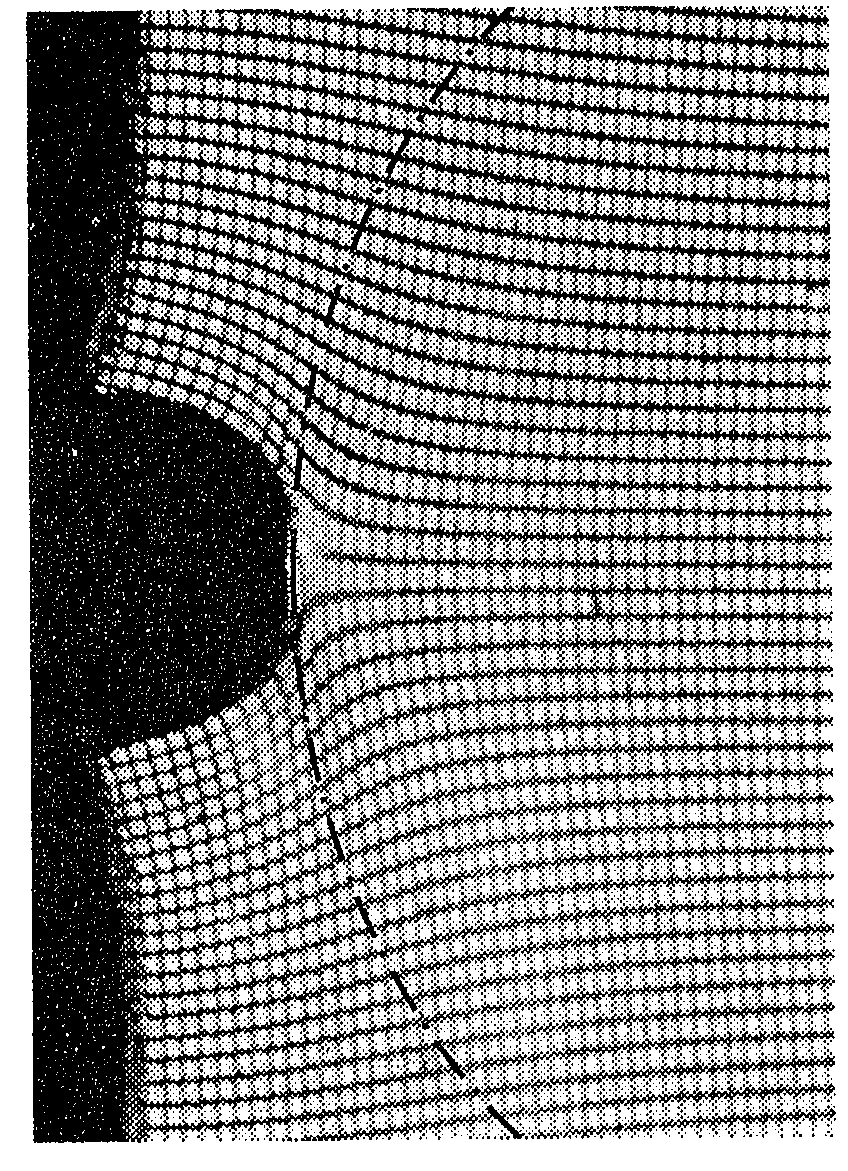
\includegraphics[width=.7\textwidth]{rubber_crack.png}
% 			\vspace{3mm}
% 			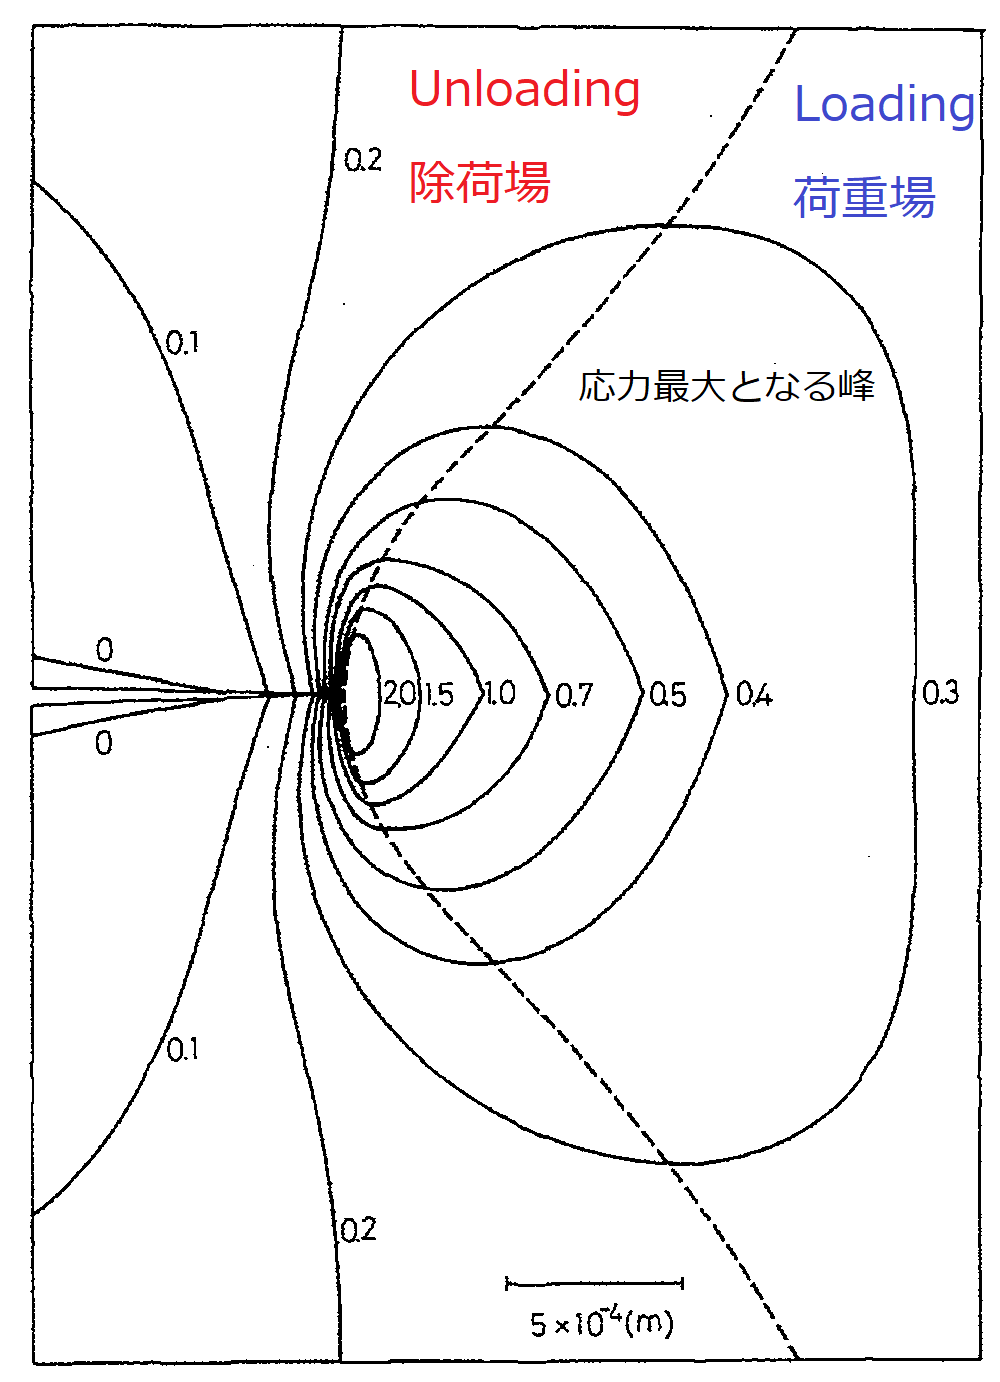
\includegraphics[width=.7\textwidth]{./crack.png}
% 		\end{columns}
% 	\end{exampleblock}
% \end{frame}


% \begin{frame}
% 	\frametitle{力学的ヒステリシス}
% 		\vspace{-2mm}
% 		\begin{exampleblock}{力学的ヒステリシス}
% 			\begin{columns}[totalwidth=\textwidth]
% 				\column{.7\textwidth}
% 					\begin{itemize}
% 						\item
% 						\textcolor{red}{Unloading} 時の応力が低下
% 						\item
% 						ヒステリシスロス$\Rightarrow$エネルギー散逸
% 					\end{itemize}
% 				\column{.3\textwidth}
% 					\centering
% 					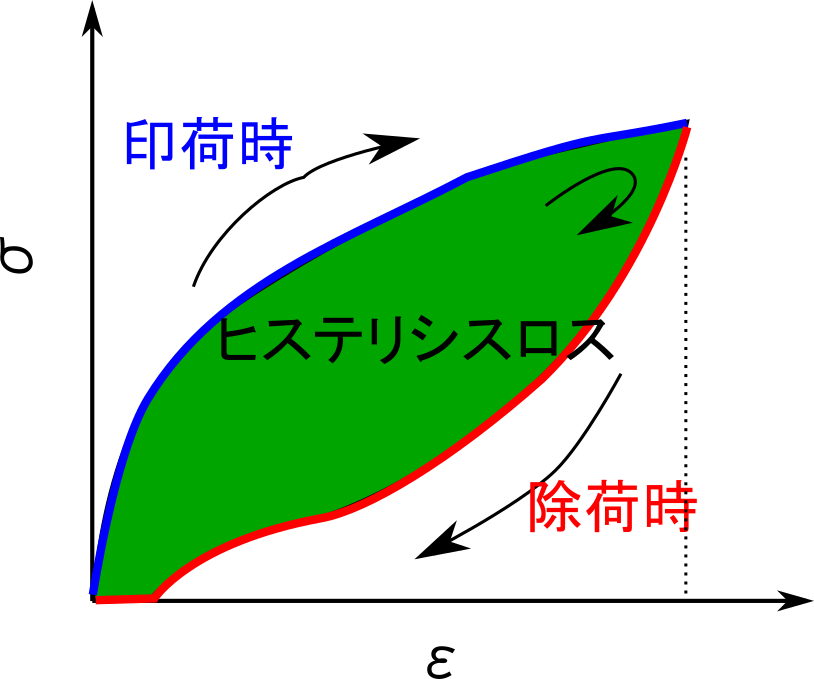
\includegraphics[width=.6\textwidth]{hysteresis_curve.png}
% 			\end{columns}
% 			\end{exampleblock}
% 			\vspace{-2mm}
% 			\begin{block}{ヒステリシス発生の起源}
% 				\begin{itemize}
% 					\item フィラーの添加効果\footnote{
% 						\scriptsize{K. A. Grosch et al. Rub. Chem. and Tech.41, 1157 (1968)}
% 					}
% 					\item フィラー近傍でのナノキャビティーの開閉\footnote{
% 						\scriptsize{H. Zhang et al. Macromol. 46, 900 (2013)}
% 					}
% 				\end{itemize}
% 			\end{block}
% 			\vspace{-2mm}
% 			\begin{alertblock}{疲労破壊も考慮すると}
% 				\begin{itemize}
% 					\item \alert{可逆的}であることが望ましい。\textcolor{blue}{$\neq$ 犠牲結合}
% 					\item 変形の周期に対応できるように、\alert{回復速度}も重要。
% 				\end{itemize}
% 			\end{alertblock}
% \end{frame}


% %%%%%%%%%%%%%%%%%


% \subsection{ゴムのモデル化}

% \begin{frame}
% 	\frametitle{ひずみ不変量}

% 	主伸張比 $\lambda$ を用いて以下のように、\\ひずみの第1不変量、第2不変量、第3不変量
% 		\begin{align*}
% 			I_1 &= \lambda_1^2 + \lambda_2^2 + \lambda_3^2 \\
% 			I_2 &= \lambda_1^2\lambda_2^2 + \lambda_2^2\lambda_3^2 + \lambda_3^2\lambda_1^2 \\
% 			I_1 &= \lambda_1^2\lambda_2^2\lambda_3^2
% 		\end{align*}

% 	どの座標系においても不変であり、\\物理的には以下のように解釈される。
% 	\begin{description}
% 		\item [ひずみの第1不変量]
% 		長さの変化量
% 		\item [ひずみの第2不変量]
% 		表面積の変化量
% 		\item [ひずみの第3不変量]
% 		体積の変化量
% 	\end{description}
% \end{frame}




% \begin{frame}
% 	\frametitle{架橋点近傍の拘束状態に基づく二つのモデル}
% 	\vspace{-3mm}
% 		\begin{columns}[totalwidth=1\textwidth]
% 			\column{.45\textwidth}
% 				\begin{block}{ストランドと架橋点}
% 					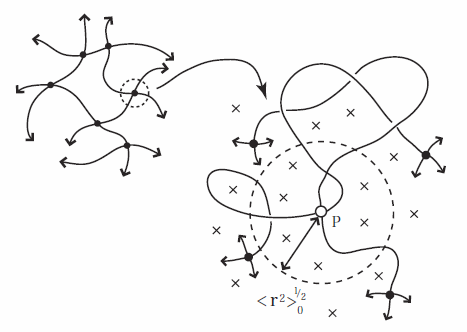
\includegraphics[width=\textwidth]{JP_vicinity.png}
% 					架橋点はストランド経由で直接連結した架橋点以外の、
% 					\alert{近接する多数のストランド(図中の×)に囲まれている。}
% 				\end{block}
% 			\column{.52\textwidth}
% 			\begin{itemize}
% 				\item \textcolor{blue}{``Affine NW Model''}\\[1mm]
% 					架橋点が巨視的変形と相似に移動。(Affine 変形)
% 					\vspace{-3mm}
% 					\footnotesize
% 					\begin{align*}
% 						&G=\nu k_B T \\
% 						&\text{$\nu$ は、ストランドの数密度}
% 					\end{align*}
% 					\normalsize
% 				\item \textcolor{red}{``Phantom NW Model''}\\[1mm]
% 					架橋点が大きく揺らぎ、ずり弾性率($G$)が低下\footnote{
% 						P. J. Flory, Proc. R. Soc. London. Series A, 351, 351 (1976)
% 					}。
% 					\vspace{-3mm}
% 					\footnotesize
% 					\begin{align*}
% 						&G={\color{red}\xi} \nu k_B T \\
% 						&{\color{red}\xi= 1 -\dfrac{2}{f}}\\
% 						&\text{$f$ は架橋点の分岐数}
% 					\end{align*}
% 			\end{itemize}
% 		\end{columns}
% \end{frame}

% % \subsection{ファントムネットワークの理論}
% \begin{frame}
% 	\frametitle{有限サイズ効果}
% 		\begin{columns}[totalwidth=1\textwidth]
% 			\column{.48\textwidth}
% 				\begin{block}{末端の壁面固定の効果}
% 				\begin{itemize}
% 					\item 壁面に末端が固定
% 						\begin{itemize}
% 							\item $n$ 本のストランド
% 							\item セグメント数: $N$
% 							\item 他端が架橋点($\bm{r}$)
% 						\end{itemize}
% 					\item 架橋点の運動性
% 						\begin{itemize}
% 							\item 壁と$N/n$ 個の短い\\ストランドと等価
% 							\item 壁の移動(変形)の影響減少
% 						\end{itemize}
% 				\end{itemize}
% 				% \vspace{-2mm}
% 				\begin{center}
% 					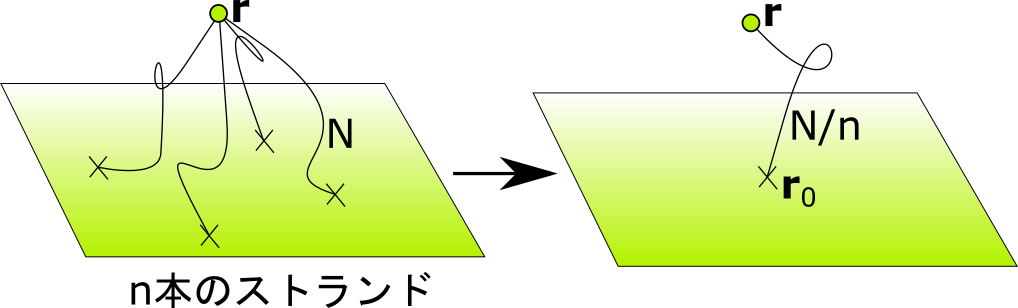
\includegraphics[width=.8\textwidth]{phantom-1.png}
% 				\end{center}
% 				\end{block}
% 			\column{.48\textwidth}
% 				\begin{exampleblock}{内部の鎖が受ける変形}
% 					\begin{itemize}
% 						\item システム内部の鎖の末端はガウス分布
% 						\item 壁面固定の末端からの変形が内部に伝達して、
% 					\end{itemize}
% 					\tiny
% 					\begin{align*}
% 						&G=\xi \nu k_BT \\
% 							&\begin{cases}
% 							\xi_{\infty} = 1-\dfrac{2}{f} \;\; \text{System}\sim \infty \\[8pt]
% 							\xi_{s} = \dfrac{f-1}{f+1} \;\; \text{Small Limit}
% 							\end{cases}
% 					\end{align*}
% 					\vspace{-3mm}
% 					\begin{center}
% 						\includegraphics[width=0.5\textwidth]{phantom.png}
% 					\end{center}
% 				\end{exampleblock}
% 		\end{columns}
% \end{frame}
% %%%%%%%%%%%%%%%%%%%%%%%%%%
% % \subsection{ファントムネットワークの振る舞い}
% \begin{frame}
% 	\frametitle{ファントムネットワークのゆらぎ}
% 		\begin{block}{ゆらぎの入ったポテンシャル}
% 			\begin{itemize}
% 				\item ストランドの末端間ベクトル $\bm{R}_{nm}$ を、\\架橋点の位置ベクトル $\bm{r}_n$ を用いて、
% 					\footnotesize
% 					\begin{equation*}
% 						\bm{R}_{nm} \equiv \bm{r}_n-\bm{r}_m
% 					\end{equation*}
% 					\normalsize
% 				\item 系のポテンシャルエネルギーは、
% 					\footnotesize
% 					\begin{equation*}
% 						U=\dfrac{k}{2} \sum_{\langle nm \rangle} \bm{R}_{nm}^2
% 					\end{equation*}
% 					\normalsize
% 				\item これは、自然長で決まる定数項と、ゆらぎに起因した第二項に分割でき、その和で以下となる。
% 					\footnotesize
% 					\begin{equation*}
% 						U=\dfrac{k}{2} \sum_{\langle nm \rangle} {\bm{R}_{nm}^{(0)}}^2 + \dfrac{k}{2} \sum_{\langle nm \rangle} \Delta \bm{R}_{nm}^2
% 					\end{equation*}
% 					\normalsize
% 			\end{itemize}
% 		\end{block}
% \end{frame}

% \begin{frame}
% 	\frametitle{ファントムネットワークのゆらぎ}
% 		\begin{block}{アンサンブル平均の 2 つの表式}
% 			\scriptsize
% 			\begin{align*}
% 				\begin{cases}
% 					\langle U \rangle = N_{strands} \dfrac{k}{2} \langle \Delta \bm{R}^2 \rangle \\
% 					\langle U \rangle = 3(N_{nodes}-1) \dfrac{1}{2} k_B T
% 				\end{cases}
% 			\end{align*}
% 			\normalsize
% 			なお、第二式は等分配側より導出した。
% 		\end{block}
% 		\begin{exampleblock}{ファントムネットワークでのゆらぎ}
% 			\begin{itemize}
% 				\item 架橋点数 $N_{nodes}$、架橋点官能基数 $f$ とすれば、
% 					\scriptsize
% 					\begin{equation*}
% 					\langle \Delta \bm{R}^2 \rangle = \dfrac{3k_B T}{k} \dfrac{2}{f} \left( 1-\dfrac{1}{N_{nodes}} \right)
% 					\end{equation*}
% 					\normalsize
% 				\item 適切な条件で、ストランドの自然長 $R_0$ を用いて、
% 					\scriptsize
% 					\begin{equation*}
% 					\color{red}
% 					\langle \Delta \bm{R}^2 \rangle = \dfrac{2}{f} R_0^2
% 					\end{equation*}
% 			\end{itemize}
% 		\end{exampleblock}
% \end{frame}


% \begin{frame}
%     \frametitle{Constrained Junction Model}
% 	\begin{exampleblock}{伸長時の緩和現象}
% 		\begin{itemize}
% 			\item 伸長時に
% 			\begin{itemize}
% 				\item ストランドに直交する他の鎖の影響が緩む
% 				\item 架橋点およびストランドへの規制が緩和
% 			\end{itemize}
% 		\end{itemize}
% 		\begin{center}
% 			\includegraphics[width=.7\textwidth]{Constrained_Juntion.pdf}

% 			P.J.Flory, J.C.P., 66 5720 (1977)
% 		\end{center}
% 	\end{exampleblock}
% \end{frame}		




% \section{ランダムネットワークについて}

% \subsection{ランダムネットワークの作成}
% \begin{frame}
% 	\frametitle{トポロジーモデルへの変換}
% 		\begin{columns}[totalwidth=\textwidth]
% 			\column{.48\textwidth}
% 				\begin{block}{実空間での初期構造}
% 					\begin{itemize}
% 						\item $2\times2\times2$ 個の\\ユニットセル
			
% 							\includegraphics[width=0.8\columnwidth]{8_per.png}

% 						\item ユニットセルから除去

% 							\includegraphics[width=0.8\columnwidth]{8_4.png}

% 					\end{itemize}
% 				\end{block}
% 		\column{.48\textwidth}
% 			\begin{exampleblock}{トポロジーモデル}
% 				分岐数を4に減じた\\トポロジーモデル

% 				\includegraphics[width=\columnwidth]{Network.png}

% 			\end{exampleblock}
% 		\end{columns}
% \end{frame}

% \begin{frame}
% 	\frametitle{それぞれの分岐数での初期構造}
% 		\begin{exampleblock}{初期構造の作成}
% 			\begin{itemize}
% 				\item \alert{実空間}で8-Chain Model で初期構造を作成。
% 				\item 所望の分岐数に\alert{ランダム}に選択した\alert{結合を除去}
% 				\item 除去したジオメトリーに対応した\alert{トポロジーモデル}
% 			\end{itemize}
% 		\end{exampleblock}
% 		\begin{columns}[totalwidth=\linewidth]
% 			\column{.48\linewidth}
% 				\begin{block}{分岐数: 3, 4, 5 分岐}
% 					\begin{itemize}
% 						\item 3 分岐では、全てが連結していない
% 						\item 4 分岐では、連結していないものもある
% 						\item 5 分岐でも二種類のみ
% 					\end{itemize}
% 				\end{block}
% 			\column{.48\linewidth}
% 				\includegraphics[width=\columnwidth]{Histgram2.png}
% 		\end{columns}
% \end{frame}

% \begin{frame}
% 	\frametitle{トポロジーモデルからのランダム性の導入}
% 		\includegraphics[width=\textwidth]{bond_exchg.png}
% \end{frame}

% \begin{frame}
% 	\frametitle{代数的連結性の分布関数}
% 		\begin{exampleblock}{サンプリング数の増加($> 1000,000$ times)}
% 			\begin{itemize}
% 				\item 3, 5分岐トポロジーモデルは、単鋒性に
% 				\item 4分岐のトポロジーモデルでは、二峰性\\
% 				サンプリング数を増やすと若干変化
% 			\end{itemize}
% 		\end{exampleblock}
% 		\begin{columns}[totalwidth=1\textwidth]
% 			\column{.33\textwidth}
% 				\begin{center}
% 					\includegraphics[width=1.2\columnwidth]{3.png}

% 					3-Chain Model
% 				\end{center}
% 			\column{.33\textwidth}
% 				\begin{center}
% 					\includegraphics[width=1.2\columnwidth]{4_1000_5000.png}

% 					4-Chain Model
% 				\end{center}
% 			\column{.33\textwidth}
% 				\begin{center}
% 					\includegraphics[width=1.2\columnwidth]{5.png}

% 					5-Chain Model
% 				\end{center}
% 		\end{columns}
% \end{frame}


% \subsection{ネットワークのトポロジー}
% \begin{frame}
% 	\frametitle{ネットワークの分岐数の処理}
% 		以下のようにノード番号を付与したネットワークを考えると、
% 			\begin{center}
% 				\includegraphics[width=4cm]{NW-4.png}
% 			\end{center}
% 		隣接行列、および、次数行列は、
% 		\begin{align*}
% 			A = \left( 
% 			\begin{array}{cccc} 
% 			0 & 1 & 1 & 1 \\ 
% 			1 & 0 & 1 & 0 \\
% 			1 & 1 & 0 & 1 \\
% 			1 & 0 & 1 & 0 
% 			\end{array} 
% 			\right) 
% 			,
% 			D = \left( 
% 			\begin{array}{cccc} 
% 			3 & 0 & 0 & 0 \\ 
% 			0 & 2 & 0 & 0 \\
% 			0 & 0 & 3 & 0 \\
% 			0 & 0 & 0 & 2 
% 			\end{array} 
% 			\right) 
% 		\end{align*}
% 		となる。
% \end{frame}

% \subsection{ラプラシアン行列}
% \begin{frame}
% 	\frametitle{ラプラシアン行列}
% 		\begin{columns}[totalwidth=1\textwidth]
% 			\column{.48\textwidth}
% 				ラプラシアン行列は、隣接行列$A$と次数行列$D$により以下のように定義される。
% 				$$
% 				L \equiv D-A
% 				$$
% 				4つのノードからなるネットワークの例であれば、
% 				$$
% 				L = \left( 
% 				\begin{array}{cccc} 
% 				3 & -1 & -1 & -1 \\ 
% 				-1 &  2 & -1 & 0 \\
% 				-1 & -1 &  3 & -1 \\
% 				-1 &  0 & -1 & 2 
% 				\end{array} 
% 				\right) 
% 				$$
% 				となり、非負の固有値。
% 			\column{.48\textwidth}
% 				グラフが非連結であるとき、%ラプラシアン行列の成分を
% 				連結した成分ごとにブロック対角化できるので、固有値 0 の重複数がグラフの連結成分ブロックの総数となる。
% 				\begin{block}{「代数的連結性」}
% 					「グラフが連結である場合、ラプラシアン行列の固有値 0 の重複数は 1」となる。\\
% 					固有値を昇順にみた時、0 に次ぐ 2 番目の固有値がグラフの連結性の強さを示す指標となり、「代数的連結性」と呼ばれる。
% 				\end{block}
% 		\end{columns}
% \end{frame}


% %%%%%%%%%%%%%%%%%%%%%%%%%%%%
% \section{その他}
% % \subsection{破壊について}

% %%%%%%%%%%%%%%%%%%%%%%%%%%%%%%


% % \subsection{以前の検討結果:規則ネットワーク構造}
% % \begin{frame}
% % 	\frametitle{規則ネットワーク構造のMDシミュレーション}
% % 	ストランド長一定の規則構造\footnote{
% % 		R.Everaers, New J. of Phys. 1, 12, 12 (1999)\\
% % 		M.Toda, H.Morita, AIP Advances, 8, 12, 125005 (2018)
% % 			}
% % 	\begin{columns}[totalwidth=\textwidth]
% % 		\column{.6\textwidth}
% % 			\begin{itemize}
% % 				\item 分岐数 
% % 					\begin{itemize}
% % 						\item 三分岐: K4 構造
% % 						\item 四分岐: ダイヤモンド構造
% % 					\end{itemize}
% % 				\item ストランド
% % 					\begin{itemize}
% % 						\item KG鎖\\LJ ポテンシャルにより、\\ \alert{排除体積効果}を導入
% % 						\item 素抜け鎖\\{\color{blue}排除体積効果を無視}
% %                         % \\$\simeq$\alert{理想鎖}
% % 					\end{itemize}
% % 			\end{itemize}
% % 		\column{.4\textwidth}
% % 			\small
% % 			\begin{itemize}
% % 				\item K4 構造

% % 				\includegraphics[width=0.6\textwidth]{K4_d.png}

% % 				\item ダイヤモンド構造

% % 				\includegraphics[width=0.6\textwidth]{dia.png}

% % 			\end{itemize}
% % 	\end{columns}
% % \end{frame}

% % \begin{frame}
% % 	\frametitle{規則ネットワーク構造での検討結果}
% % 		\small
% % 		\begin{alertblock}{規則ネットワーク構造の振る舞い}
% % 			\begin{itemize}
% % 				\item 一軸伸長で、\alert{アフィンネットワークモデルの挙動}を示した
% % 					\begin{itemize}
% % 						\item \alert{分岐数、ストランドの性質(KG、素抜け)}によらず
% % 				%	\item
% % 				%	伸びきり効果をほぼ再現
% % 					\end{itemize}
% % 				\item 応力緩和で、主緩和がラウスモードの最長緩和時間程度
% % 				\item 主緩和近傍に大きなエネルギー散逸($\tan \delta > 1$)を確認
% % 			\end{itemize}
% % 		\end{alertblock}
% % 		\begin{columns}[totalwidth=1\textwidth]
% % 			\column{.32\textwidth}
% % 				\scriptsize
% % 				一軸伸長結果
% % 				% \vspace{-2mm}
% % 				\includegraphics[width=0.9\textwidth]{SS_Kuhn.pdf}
% % 			\column{.32\textwidth}
% % 				\scriptsize
% % 				応力緩和挙動
% % 				% \vspace{-2mm}
% % 				\includegraphics[width=0.9\textwidth]{Gt_loglog.pdf}
% % 			\column{.32\textwidth}
% % 				\scriptsize
% % 				粘弾性スペクトル
% % 				% \vspace{-2mm}
% % 				\includegraphics[width=\textwidth]{N_44_Freq_Sweep.pdf}
% % 		\end{columns}
% % \end{frame}

% % \subsection{規則構造でのアフィン性}

% \begin{frame}
% 	\frametitle{規則構造でのアフィン性}
% 		\vspace{-2mm}
% 		\begin{columns}[totalwidth=\linewidth]
% 			\column{.5\linewidth}
% 				\begin{block}{規則構造の特徴}
% 					\begin{itemize}
% 						\item 規則構造においては、\\結節点の\alert{連結性は等価}
% 							\begin{itemize}
% 								% \item それぞれの結節点の\\ゆらぎも等価
% 								\item 結節点は規則構造の\\平均位置に拘束
% 							\end{itemize}
% 						\item 巨視的な変形後
% 							\begin{itemize}
% 								\item 結節点の\alert{平均位置が\\アフィン移動}
% 								\item ゆらぎの異方性も類似
% 							\end{itemize}
% 					\end{itemize}
% 				\end{block}
% 			\column{.45\linewidth}
% 				規則構造の模式図
% 				\vspace{2mm}
% 				\includegraphics[width=.9\columnwidth]{reglar_NW_2.png}
% 		\end{columns}
% 		\vspace{-2mm}
% 		\begin{alertblock}{規則ネットワークの特徴}
% 			\begin{itemize}
% 				\item 分岐数、ストランドの性質(KG、素抜け)によらず\\ \alert{アフィンネットワークモデルの挙動}
% 				\item {緩和モードも単純}
% 			\end{itemize}
% 		\end{alertblock}
% \end{frame}

% \subsection{ランダムネットワークの振る舞い}


% \begin{frame}
% 	\frametitle{「す抜け鎖」での一軸伸長}
% 		\begin{exampleblock}{一軸伸長:Z軸方向に二倍に伸長}
% 			\begin{itemize}
% 				\item ストランド:す抜け鎖
% 				\item 四分岐ランダムネットワークモデル
% 				\item 初期長さ:$|\bm{R_z}| = 3.46$
% 				\item 伸長後:$|\bm{R_z}| = 5.62 \Leftarrow$ \alert{二倍には伸びていない}
% 			\end{itemize}
% 		\end{exampleblock}
% 		\begin{columns}[totalwidth=\linewidth]
% 			\column{.48\linewidth}
% 				\includegraphics[width=1.1\columnwidth]{4chain_E2E_init.png}
% 			\column{.48\linewidth}
% 				\includegraphics[width=1.1\columnwidth]{Expand_4_Strand_histgram.png}
% 		\end{columns}
% \end{frame}

% \subsection{絡み合いの評価}

% \begin{frame}
% 	\frametitle{ネットワーク構造でのG1-cord}
% 		\begin{center}
% 			\includegraphics[width=.8\textwidth]{g1cord.png}
% 		\end{center}
% \end{frame}

% \backupend

\end{document}
